\documentclass[xcolor=table,usenames,dvipsnames]{lib/bredelebeamer}

\usepackage{multirow}
\usepackage{listings,pdfpages,tabulary}

\makeatletter
\let\beamer@writeslidentry@miniframeson=\beamer@writeslidentry
\def\beamer@writeslidentry@miniframesoff{%
    \expandafter\beamer@ifempty\expandafter{\beamer@framestartpage}{}
    {
        \clearpage\beamer@notesactions%
    }
}
\newcommand*{\miniframeson}{\let\beamer@writeslidentry=\beamer@writeslidentry@miniframeson}
\newcommand*{\miniframesoff}{\let\beamer@writeslidentry=\beamer@writeslidentry@miniframesoff}
\makeatother

\setbeamercolor{block title}{use=structure,fg=white,bg=structure.fg!75!black}
\setbeamercolor{block body}{parent=normal text,use=block title,bg=block title.bg!10!bg}

\title[PhD Thesis defense]{Tools for code and countermeasures analysis against multiple faults attacks}
\subtitle{PhD Thesis defense}
\subject{PhD Thesis defense - Boespflug Etienne}

\author[Etienne Boespflug]{Etienne Boespflug}

\date{April 28, 2023}

\logo{
    
\includegraphics[scale=0.08]{img/logo_VERIMAG.png}
}

\newcommand{\ignore}[1]{} % inline comment simulation. 

\begin{document}

\begin{frame}
    \titlepage
    \begin{center}
        {\small Supervised by Marie-Laure Potet and Laurent Mounier}
    \end{center}
    
    \vspace{0.1cm}
    
    \begin{center}
        \noindent \tiny 
        \begin{tabular}{llcl}
            \textit{Rapporteurs :}	& Karine \textsc{Heydemann}		& - & Maître de conférences (Sorbonne Université)\\
                    & Julien \textsc{Signoles}		& - & Ingénieur de recherche (CEA Saclay)\\
            \textit{Directeur :}	& Marie-Laure \textsc{Potet}		& - & Professeur des universités (Grenoble INP)\\
            \textit{Examinateurs :}   & Vincent \textsc{Beroulle}          & - & Professeur des universités (Grenoble INP)\\
                        & Thomas \textsc{Jensen}			& - & Directeur de recherche (INRIA de Rennes)\\
            \textit{Invités :}		& David \textsc{Féliot}		& - & Ingénieur (CEA Leti)\\
                        & Laurent \textsc{Mounier}		& - & Maître de conférences (Université Grenoble Alpes)\\
        \end{tabular}
        \vfill
        {\tiny Supported by SECURIOT-2-AAP FUI 23, by ANR-15-IDEX-02 and LabEx PERSYVAL-Lab (ANR-11-LABX-0025-01)}
    \end{center}

\end{frame}

\definecolor{darkblue}{rgb}{0,0,0.5}
\definecolor{dkgreen}{rgb}{0,0.6,0}
\definecolor{gray}{rgb}{0.5,0.5,0.5}
\definecolor{mauve}{rgb}{0.58,0,0.82}

\lstdefinestyle{customc}{
    numbers=left,
    belowcaptionskip=1\baselineskip,
    breaklines=true,
    xleftmargin=\parindent,
    language=C,
    showstringspaces=false,
    basicstyle=\tiny\ttfamily,
    keywordstyle=\bfseries\color{dkgreen},
    commentstyle=\itshape\color{red},
    identifierstyle=\color{blue},
    stringstyle=\color{mauve},
    numberstyle=\ttfamily
}

\lstdefinestyle{custompython}{
    language=Python, 
    commentstyle=\color{dkgreen},
    keywordstyle=\color{red},
    identifierstyle=\color{blue},
    emph={testfunc,print,src},
    numberstyle=\tiny\color{gray},
    stringstyle=\color{mauve},
    basicstyle=\tiny\ttfamily,
    breakatwhitespace=false,         
    breaklines=true,                 
    captionpos=b,                    
    keepspaces=true,                 
    numbers=left,                    
    numbersep=5pt,                  
    showspaces=false,                
    showstringspaces=false,
    showtabs=false,                  
    tabsize=2
}

\setcounter{tocdepth}{1}
\AtBeginSection[]
{
\begin{frame}<beamer>[noframenumbering, plain]
  \frametitle{Outline}
  \tableofcontents[currentsection]
\end{frame}
}

\section{Context}
\subsection{Fault injection}

% FI
\begin{frame}[fragile]{Fault Injection}
\vfill
{
\small
\begin{columns}
    \begin{column}{0.4\textwidth}
     
        \vfill
        \textbf{Fault-injection attacks} %\cite{Boneh/EUROCRYPT97, Barenghi/IEEE2012}
        \begin{itemize}
            \item[]
            \item Lasers% \cite{Roscian/FDTC13, Colombier/HOST19}
            \item Electromagnetic pulses %\cite{Poucheret/FDTC11}
            \item Temperature %\cite{Hutter/ICSCRAA13}
            \item Power \& clock glitches% \cite{Schmidt/FDTC09, Yuce/HSS16}
            \item Software induced %\cite{Kim/ACM14, Seaborn/BH15}
            \item[]
        \end{itemize}
    
    \end{column}
    \begin{column}{0.6\textwidth}
        \only<1>{     
            \begin{figure}
                \centering
                \caption{Laser fault injection bench [1]}
                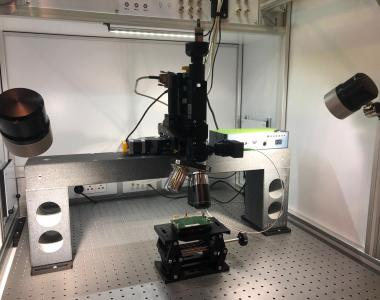
\includegraphics[width=0.67\textwidth]{img/s-lms4.jpg}
            \end{figure}
        }
        \only<2-> {
            \begin{figure}
                \centering
                \caption{Rowhammer principle [2]}
                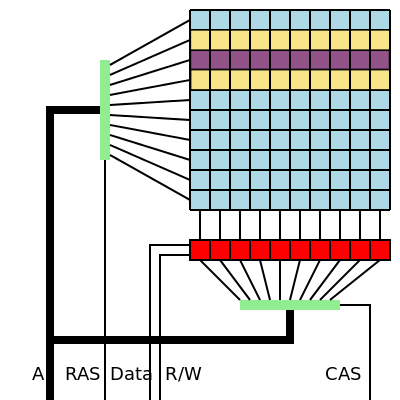
\includegraphics[width=0.55\textwidth]{img/Row_hammer.svg.png}
            \end{figure}
        }
    \end{column}
\end{columns}
\vfill
        \textit{Goal}: modify device behavior/state to break security property and gain advantage
}
\end{frame}

% Verify_pin
\begin{frame}[fragile]{\texttt{verify\_pin} program}
    \begin{columns}
        \begin{column}{0.55\textwidth}
            \begin{small}
                PIN verification program from FISSC \cite{Dureuil/PPLCC16} collection                
            \end{small}
            
            \vspace{0.2cm}
            
            \lstset{style=customc}
            \begin{lstlisting}
bool compare(uchar* a1, uchar* a2, size_t size)
{
    bool ret = true;
    size_t i = 0; 
    for(; i < size; i++)
        if(a1[i] != a2[i])
            ret = false;
        
    return ret;
}

bool verify_pin(uchar* user_pin) {
    if(try_counter > 0)  
        if(compare(user_pin, card_pin, PIN_SIZE)) {
            // Authentication
            try_counter = 3;
            return true;
        } else {
            try_counter--;
            return false;
        }
    return false;
}
            \end{lstlisting}	
        	\vfill
        \end{column}
        \begin{column}{0.45\textwidth}
        	\begin{small}
                 \begin{itemize}
                     \item Compare user PIN against the card's one in constant time
                     \item[] 
                     \item \textit{Attack objective:} being authenticated with a false PIN
                     \item[]
                 \end{itemize}
    	    \end{small}
            \vfill
        \end{column}
    \end{columns}
\end{frame}

% Fault example
\begin{frame}[fragile]{Faults injection - Example on \texttt{verify\_pin}}
    \begin{columns}
        \begin{column}{0.55\textwidth}
            \begin{small}
                PIN verification program from FISSC \cite{Dureuil/PPLCC16} collection                
            \end{small}
            
            \vspace{0.2cm}
            
            \lstset{style=customc, escapeinside={(*}{*)}}
            \begin{lstlisting}
bool compare(uchar* a1, uchar* a2, size_t size)
{
    bool ret = true;
    size_t i = 0; 
    for(; (*{\color{red} i < size}*); i++) // Fault: avoid the loop
        if(a1[i] != a2[i])
            ret = false;
        
    return ret;
}

bool verify_pin(uchar* user_pin) {
    if(try_counter > 0)  
        if(compare(user_pin, card_pin, PIN_SIZE)) {
            // Authentication
            try_counter = 3;
            return true;
        } else {
            try_counter--;
            return false;
        }
    return false;
}
            \end{lstlisting}	
        	\vfill
        \end{column}
        \begin{column}{0.45\textwidth}
        	\begin{small}
                 \begin{itemize}
                     \item Fault model: modelisation of the faults to be injected
                     \item[] $\rightarrow$ ex: \textbf{Test inversion}: inverse the branch taken during conditional branching
                     \item[]
                 \end{itemize}
    	    \end{small}
            \vfill
        \end{column}
    \end{columns}
\end{frame}

% CM example 
\begin{frame}[fragile, noframenumbering]{Faults injection - Example on \texttt{verify\_pin}}
    \begin{columns}
        \begin{column}{0.55\textwidth}
            \begin{small}
                PIN verification program from FISSC \cite{Dureuil/PPLCC16} collection                
            \end{small}
            
            \vspace{0.2cm}
            
            \lstset{style=customc, escapeinside={(*}{*)}}
            \begin{lstlisting}
bool compare(uchar* a1, uchar* a2, size_t size)
{
    bool ret = true;
    size_t i = 0; 
    for(; (*{\color{red} i < size}*); i++) // Fault
        if(a1[i] != a2[i])
            ret = false;
            
    if(i != size) // Countermeasure
        killcard(); 
        
    return ret;
}

bool verify_pin(uchar* user_pin) {
    if(try_counter > 0)  
        if(compare(user_pin, card_pin, PIN_SIZE)) {
            // Authentication
            try_counter = 3;
            return true;
        } else {
            try_counter--;
            return false;
        }
    return false;
}
            \end{lstlisting}	
        	\vfill
        \end{column}
        \begin{column}{0.45\textwidth}
        	\begin{small}
                 \begin{itemize}
                     \item Fault model: modelisation of the faults to be injected
                     \item[] $\rightarrow$ ex: Test inversion: inverse the branch taken during conditional branching
                     \item[]
                     \item \textbf{Software countermeasures (program transformations) can be placed to protect against faults}
                     \item[]
                 \end{itemize}
    	    \end{small}
            \vfill
        \end{column}
    \end{columns}
\end{frame}

% CM attack
\begin{frame}[fragile, noframenumbering]{Faults injection - Example on \texttt{verify\_pin}}
    \begin{columns}
        \begin{column}{0.55\textwidth}
            \begin{small}
                PIN verification program from FISSC \cite{Dureuil/PPLCC16} collection                
            \end{small}
            \vspace{0.2cm}
            
            \lstset{style=customc, escapeinside={(*}{*)}}
            \begin{lstlisting}
bool compare(uchar* a1, uchar* a2, size_t size)
{
    bool ret = true;
    size_t i = 0; 
    for(; (*{\color{red} i < size}*); i++) // Fault 1
        if(a1[i] != a2[i])
            ret = false;
            
    if((*{\color{red} i != size}*)) // Fault 2 => countermeasure attack
        killcard(); 
        
    return ret;
}

bool verify_pin(uchar* user_pin) {
    if(try_counter > 0)  
        if(compare(user_pin, card_pin, PIN_SIZE)) {
            // Authentication
            try_counter = 3;
            return true;
        } else {
            try_counter--;
            return false;
        }
    return false;
}
            \end{lstlisting}	
        	\vfill
        \end{column}
        \begin{column}{0.45\textwidth}
        	\begin{small}
                 \begin{itemize}
                     \item Fault model: modelisation of the faults to be injected
                     \item[] $\rightarrow$ ex: Test inversion: inverse the branch taken during conditional branching
                     \item[]
                     \item Software countermeasures (program transformations) can be placed to protect against faults
                     \item[] \textbf{multiples faults $\rightarrow$ countermeasures themselves can be attacked }
                     \item[]
                 \end{itemize}
    	    \end{small}
            \vfill
        \end{column}
    \end{columns}
\end{frame}


\subsection{Multiple faults}

\begin{frame}[fragile]{Multiple Faults}
\vfill
    State of the art attacks combine several faults to achieve their goal. % \cite{kim2007fault, Natella/ACM16}
    %Wookey Attack [Wookey 22]: first fault invalidate countermeasures, second exploit a buffer overflow vulnerability.
    \vspace{0.2cm}
    Most robustness evaluation tools consider only single fault
    
    {\small    
        \vspace{0.3cm}
        \
        \begin{itemize}
            \item Need to help developer and auditor in multiple faults
            \item []
            \item Standard analysis cannot be trivially applied
            \item[] $\rightarrow$ faults can induce modification in the CFG or the data flow
            \item []
            \item \onslide<2->{Exploration of faulted execution is subject to \textit{combinatory explosion} of paths due to faults}
            \item []
            \item []
        \end{itemize}
        
        \onslide<3->{    
            \begin{block}{\textbf{Probl. 1}}
                Need of automated tools to evaluate programs against multiple faults attacks
            \end{block}
        }
    }
\end{frame}


%%%%%%%%%%%%%%%%%%%%%%%%%%%%%%%%%%%%%%%%%%%%%%%%%%%%%%%%%%%%%%%%%%%%%%%%
\begin{frame}[fragile] \frametitle{Robustness evaluation in multiple faults} 
    \begin{small}
        \begin{itemize}
            \item Comparing the robustness of different protected versions of a program is not trivial
            \item [] $\Rightarrow$ \textit{attack surface paradox [Dureuil 2016]}: countermeasure can add attack surface to the code
            \item [] 
            \item How to count attacks in case of multiple faults ?
            \onslide<2-> {\item [] $\Rightarrow$ Which program is the most secure ?}
        \end{itemize}

        \begin{tiny}
            \centering
            \only<2>{
                \begin{table}[htb]
                    \setlength\tabcolsep{4pt}
                    \begin{tabular}{|l|l|c|c|c|c|c|c|c|}
                        \hline
                        \texttt{verify\_pin} version (from FISSC \cite{Dureuil/PPLCC16}) & countermeasures & 0-faults & 1-fault & 2-faults & 3-faults & 4-faults \\
                        \hline
                        vp\_0  \hfil & $\emptyset$ \hfil & 0     & 3 & 0  & 0  & 1 \\
                        \hline
                        vp\_1  \hfil & HB \hfil & 0     & 2 & 0  & 0  & 1 \\
                        \hline
                        vp\_2  \hfil & HB+FTL\hfil & 0     & 2 & 1  & 0  & 1 \\
                        \hline
                        vp\_3 \hfil &  HB+FTL+INL\hfil & 0     & 2 & 1  & 0  & 1 \\
                        \hline
                        vp\_4  \hfil & FTL+INL+DPTC+PTCBK+LC\hfil & 0     & 2 & 0  & 1  & 1 \\
                        \hline
                        vp\_5  \hfil & HB+FTL+DPTC+DC\hfil & 0     & 0 & 4  & 4  & 1 \\
                        \hline
                        vp\_6  \hfil & HB+FTL+INL+DPTC+DT \hfil & 0     & 0 & 3  & 0  & 1 \\
                        \hline
                        vp\_7  \hfil & HB+FTL+INL+DPTC+DT+SC\hfil & 0     & 0 & 2  & 0  & 1 \\
                        \hline
                    \end{tabular}
                \end{table}
            }
            \only<3->{
                \begin{table}[htb]
                    \setlength\tabcolsep{4pt}
                    \begin{tabular}{|l|l|c|c|c|c|c|c|c|}
                        \hline
                        \texttt{verify\_pin} version (from FISSC \cite{Dureuil/PPLCC16}) & countermeasures & 0-faults & 1-fault & 2-faults & 3-faults & 4-faults \\
                        \hline
                        vp\_0  \hfil & $\emptyset$ \hfil & 0     & 3 & 0  & 0  & 1 \\
                        \hline
                        vp\_1  \hfil & HB \hfil & 0     & 2 & 0  & 0  & 1 \\
                        \hline
                        vp\_2  \hfil & HB+FTL\hfil & 0     & 2 & 1  & 0  & 1 \\
                        \hline
                        vp\_3 \hfil &  HB+FTL+INL\hfil & 0     & 2 & 1  & 0  & 1 \\
                        \hline
                        \textbf{vp\_4}  \hfil & FTL+INL+DPTC+PTCBK+LC\hfil & \textbf{0}     & \textbf{2} & \textbf{0}  & 1  & 1 \\
                        \hline
                        \textbf{vp\_5}  \hfil & HB+FTL+DPTC+DC\hfil & \textbf{0}     & \textbf{0} & \textbf{4}  & 4  & 1 \\
                        \hline
                        vp\_6  \hfil & HB+FTL+INL+DPTC+DT \hfil & 0     & 0 & 3  & 0  & 1 \\
                        \hline
                        vp\_7  \hfil & HB+FTL+INL+DPTC+DT+SC\hfil & 0     & 0 & 2  & 0  & 1 \\
                        \hline
                    \end{tabular}
                \end{table}
            }
            \onslide<2-> {
                Legend:
                \begin{columns}
                    \begin{column}{0.5\textwidth}
                        \begin{itemize}
                            \item HB: hardened booleans
                            \item FTL: fixed time loops
                            \item INL: inlined function
                            \item PTC: try counter decremented first
                            \item PTCBK: try counter backup
                        \end{itemize}  
                    \end{column}
                    \begin{column}{0.5\textwidth}
                        \begin{itemize}
                            \item DC: double call
                            \item LC: loop counter verification
                            \item SC: step counter
                            \item DT: double test
                            \item CFI: control flow integrity \cite{Lalande/ESORICS14}
                        \end{itemize}  
                    \end{column}
                \end{columns}  
            }
        \end{tiny}

        \onslide<4->{
        \begin{columns}
            \begin{column}{0.8\textwidth}
                \begin{block}{\textbf{Probl. 2}}
                    How to evaluate programs and countermeasures in multiple-fault context ?
                \end{block}
            \end{column}
        \end{columns}
        }
    
    \vfill
    \end{small}
\end{frame}

\begin{frame}[fragile]{Countermeasures evaluation challenge in multiple faults}
\vfill
    {\small
        \begin{itemize}
            \item Try-and-error approaches are unsuitable for multi-faults
            \item[] $\rightarrow$ countermeasures themselves can be attacked
            \item [] $\rightarrow$ brute-forcing all countermeasures combinations is unrealistic
        \end{itemize}
    
        \begin{block}{
            \textbf{Probl. 3}}
            How to help to place countermeasures and give guarantees on the protected program in multiple faults context ?
        \end{block}
    
        \onslide<2-> {    
            \begin{itemize}
            \item[]
                \item $\rightarrow$ most tools use systematic (everywhere) placement approach
            \end{itemize}
            
            \begin{block}{\textbf{Probl. 4}}
            How to ensure that all added countermeasures are necessary ?
            \end{block}
        }
    }
\end{frame}

\subsection{Contributions}

\begin{frame}[fragile]{Contributions of this Thesis}
\vfill
    \begin{small}
        \begin{columns}
            \begin{column}{0.5\textwidth}    
                \textbf{Contributions}:
                \begin{itemize}
                    \item[]
                    \item Extension of the tool Lazart and of robustness analysis for multiple faults
                    \item [] $\rightarrow$ Problematic \textit{P1}, \textit{P2}
                    \item[]
                    \item \onslide<2->{Isolation analysis and placement algorithms}
                    \item[] \onslide<2->{$\rightarrow$ Problematic \textit{P2}, \textit{P3}}
                    \item []
                    \item \onslide<3->{Optimization of detector-based countermeasures}
                    \item [] \onslide<3->{$\rightarrow$ Problematic \textit{P2}, \textit{P4}}
                    \item[] 
                \end{itemize}
                
                \vfill
            
            \end{column}
            \begin{column}{0.5\textwidth}
                \textbf{Problematics:}
                \begin{itemize}
                    \item  \textit{P1}: Multi-faults tools
                    \item  \textit{P2}: Countermeasures evaluation / comparison
                    \item  \textit{P3}: Countermeasures placement
                    \item  \textit{P4}: Countermeasures necessity
                    \item[] 
                \end{itemize}
                
            \end{column}
        \end{columns}        
    \end{small}
\end{frame}


\section{The Lazart tool}

\subsection{Lazart and robustness evaluation tools}

\begin{frame}[fragile]{Lazart}
\vfill
{\small

    \begin{figure}
        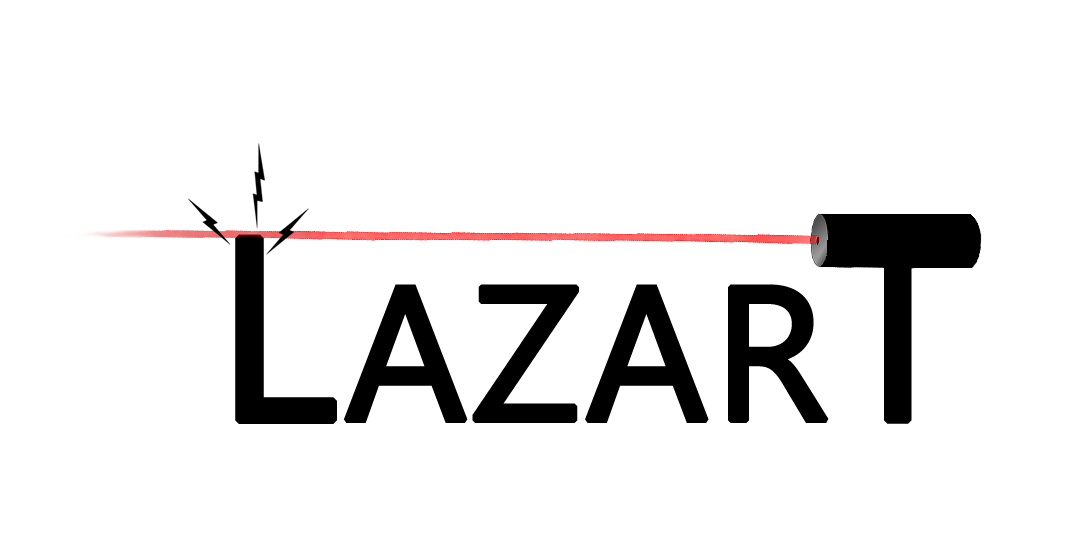
\includegraphics[scale=0.21]{img/lazart-logo-red.png}
    \end{figure}
    
    Lazart \cite{potet2014lazart} is an LLVM-level multi-fault robustness evaluation tool based on Dynamic-Symbolic Execution (KLEE)
    \begin{itemize}
        \item[] $\rightarrow$ Help developer to develop secure code
        \item[] $\rightarrow$ Help auditor to find vulnerabilities
        \item[] $\rightarrow$ Help for evaluation of countermeasures schemes
    \end{itemize}

    \vspace{0.8cm}
    
    \begin{columns}
        \begin{column}{0.5\textwidth}
            \onslide<2->{   \textbf{Handling multiple faults}:
                \begin{itemize}
                    \item Support for fault models combination
                    \item Fine description of fault space
                    \item Notion of redundancy and equivalence
                    \item[] 
                \end{itemize}
            }
        \end{column}
        \begin{column}{0.5\textwidth} 
            \onslide<3->{\textbf{Fault models}
                \begin{itemize}
                    \item Test/Branch inversion
                    \item Data mutation (\texttt{load}) (symbolic)
                    \item Jump (user-defined)
                \end{itemize}
                $\rightarrow$ cover most of high-level fault models
            }
            \vfill
    
        \end{column}
    \end{columns}
}
\end{frame}



\subsection{Principles}

\begin{frame}[fragile]{DSE and Fault Injection attacks}
\vfill
{\small

    An \textit{Injection Point} (IP) is mutated using a \textit{symbolic boolean} determining if an injection occurs, forking execution into the nominal and faulted behavior
 
    \begin{columns}   
        \begin{column}{0.5\textwidth}
            \lstset{language=C,style=customc, caption={Nominal behavior},label=lst:symbolic-ip-nominal, showlines=true}
            \begin{lstlisting}7
normal_behavior()






            \end{lstlisting}  
        \end{column}
        \begin{column}{0.5\textwidth}
            \lstset{language=C,style=customc, caption={Fault behavior},label=lst:symbolic-ip-fault, escapeinside={(*}{*)}}
            \begin{lstlisting}[label=lst-symbool]
(*{\color{mauve}inject}*) = symbolic_bool()
if (*{\color{mauve}inject}*) (*{\color{dkgreen}and}*) (*{\color{mauve}\_fault\_count}*) <= 
        (*{\color{mauve}\_fault\_limit}*):
    (*{\color{mauve}\_fault\_count}*)++
    faulted_behavior()
else:
    normal_behavior()
            \end{lstlisting}  
        \end{column}
    \end{columns}

    \begin{itemize}
        \item[] Only faults (+ values) and some entries (user-defined) are symbolic
        \item[]
    \end{itemize}

    \onslide<2>{
        \begin{itemize}
            \item Dynamic Symbolic Execution = Symbolic Execution + concretization
            \item[] $\rightarrow$ \textit{correct} (except for some concretizations)
            \item[] $\rightarrow$ not guaranteed to be \textit{complete} on path enumeration
        \end{itemize}
        
        $\rightarrow$ Lazart tries to give as much information as possible (timeout, coverage, errors...)
    }
}
\end{frame}

\subsection{Lazart's analysis}

\begin{frame}[fragile] \frametitle{Attack analysis - \texttt{verify\_pin}}
{\small
    \begin{columns}
        \begin{column}{0.60\textwidth}
            \begin{itemize}
                \item Analysis parameters:
                \item[]
                \begin{itemize}
                	\item \textbf{Inputs}: Incorrect PIN
                	\item \textbf{Attack objective}: being authenticated with a false PIN
                	\item \textbf{Fault model}: up to N \textit{test inversions}
                 \item[]
                \end{itemize}
            \end{itemize}        
            
            \begin{center}
                \begin{table}[]
                    \begin{tabular}{|l|l|l|l|l|l|}
                    \hline
                    \rowcolor[HTML]{C0C0C0} 
                    Fault limit (N)                           & 0                         & 1                         & 2                         & 3                          & 4                          \\ \hline
                    \rowcolor[HTML]{FFCCC9} 
                    \cellcolor[HTML]{C0C0C0}Attacks & \cellcolor[HTML]{9AFF99}0 & 1                         & 5                         & 10  & 11                          \\ \hline
                    \end{tabular}
                \end{table}
            \end{center}

            \onslide<2->{
                \begin{itemize}
                    \item[]
                    \item A successful 2-order attack (right) inverts the loop's condition {\color{Red}i < size} and the later check \\{\color{Red}if(i != size) killcard();}
                    \item[]
                \end{itemize}
            }
            
            \onslide<3>{
                \begin{itemize}
                    \item [] $\rightarrow$ How to simplify the attacks presented to the user in multiple faults ?
                \end{itemize}
            }
        \end{column}
        
        \onslide<2->{
            \begin{column}{0.48\textwidth}
                \begin{figure}
                        \caption{The 2-faults attack (Test Inversion)}
                    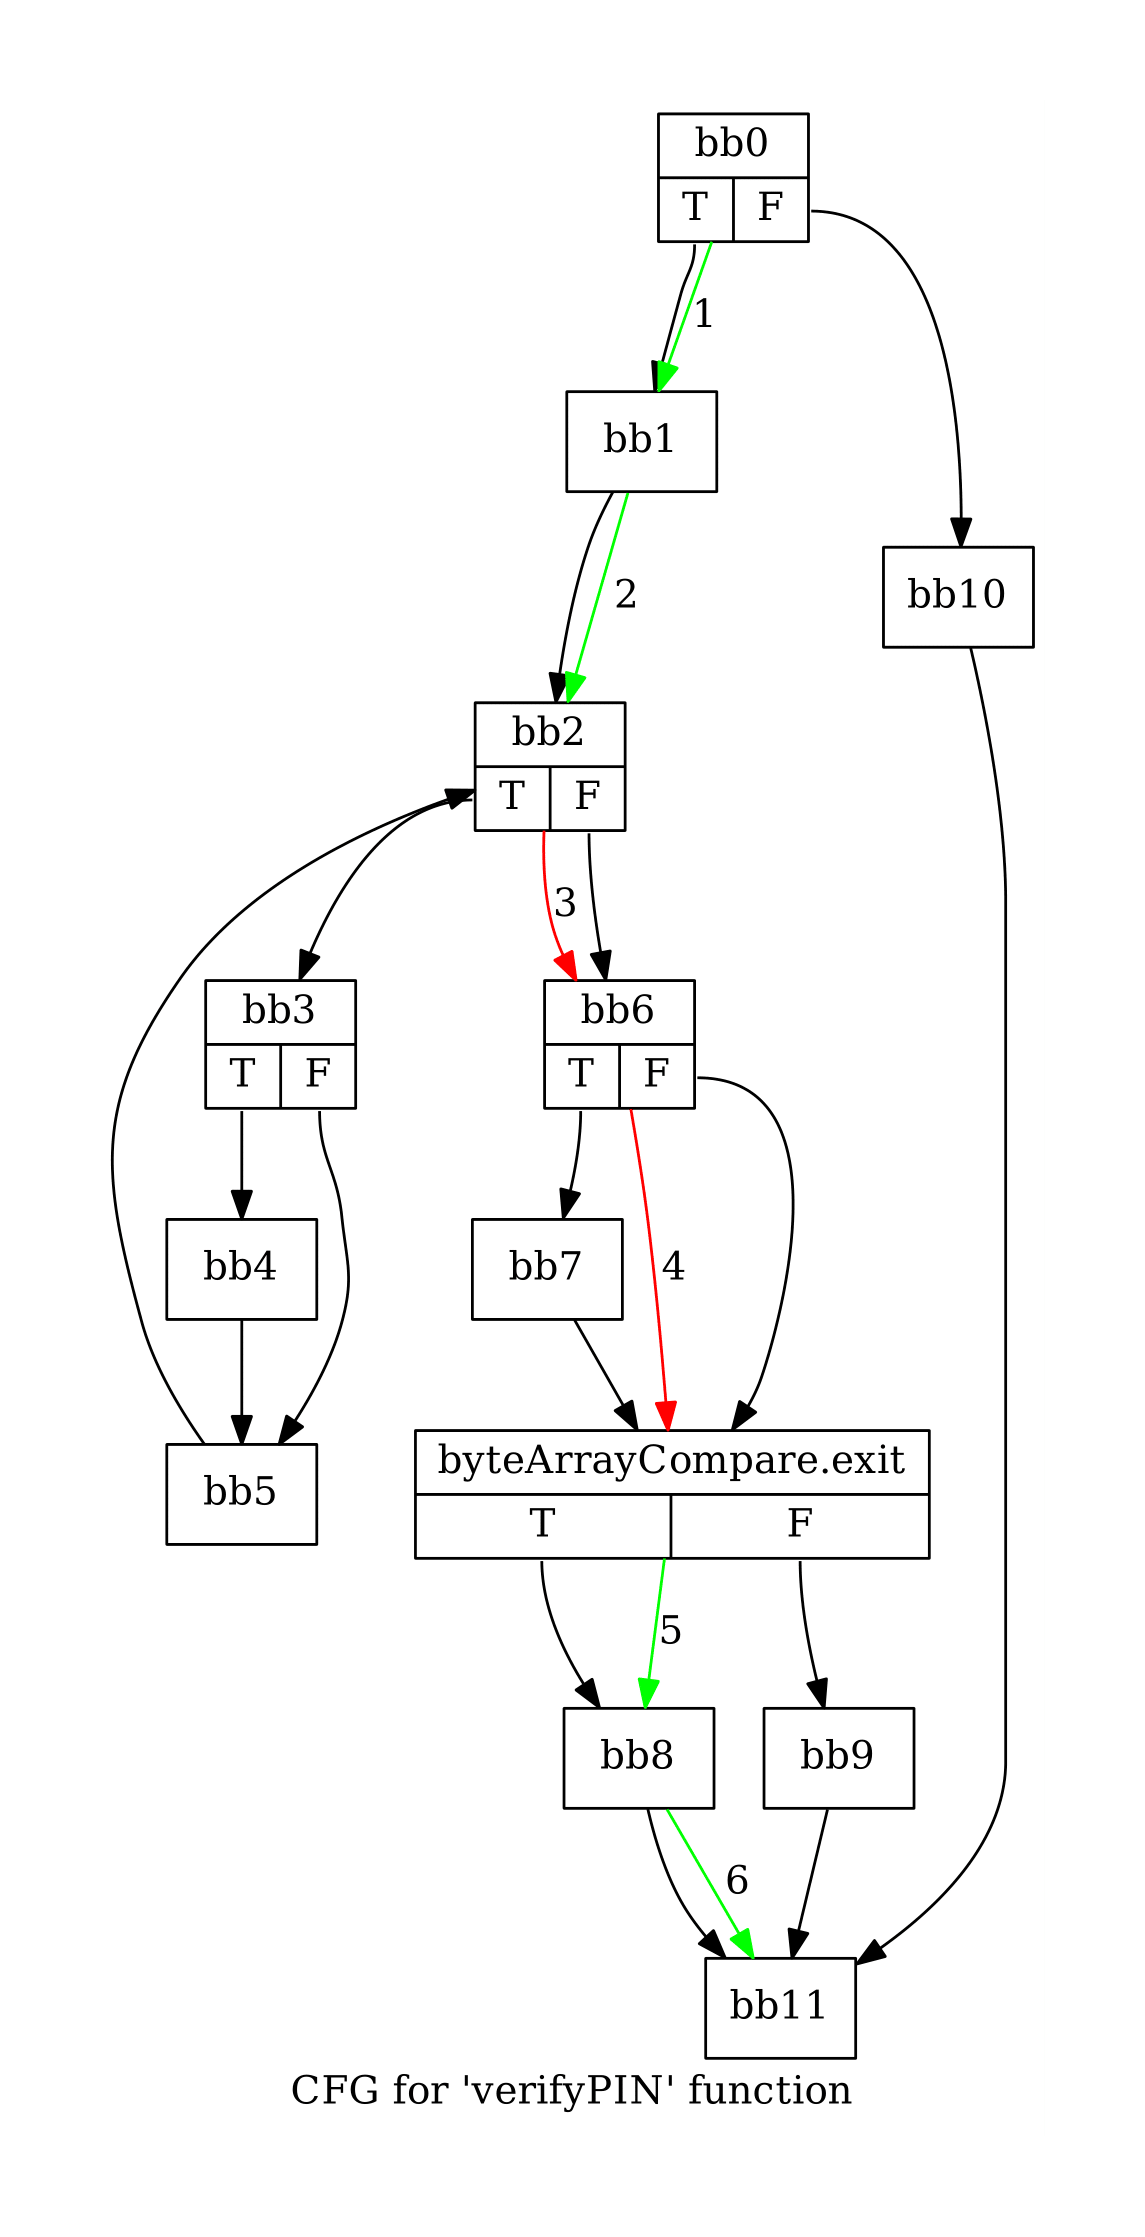
\includegraphics[scale=0.08]{img/o2-ti-atk.png}
                \end{figure}
            \end{column}
        }
        \end{columns}
    }
\vfill
\end{frame}

\begin{frame}[fragile]{Redundancy / Equivalence}
\vfill
{\tiny
    {\small Attack traces are represented as a sequence of \textit{nominal} and \textit{faulted} transitions}

    \only<1-2>{
        \begin{itemize}
            \item[]
            \item \textbf{Redundancy} and \textbf{equivalence} aims to filter attacks for the user in multiple faults
            \item[]
        \end{itemize}
    
        \begin{definition}[Redundancy prefix]
            An attack $a'$ is \textit{redundant by prefix} wrt an attack $a$ if the word of faulted transition of $a$ is a \textbf{proper prefix} of the faulted transition word of $a'$ 
        \end{definition}

        \begin{figure}
            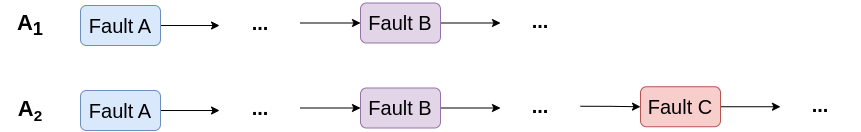
\includegraphics[scale=0.32]{img/red-prefix.png}
        \end{figure}
        \vfill
    }
    
    \only<2>{
        \begin{definition}[Redundancy subword]
            An attack $a'$ is \textit{redundant by subword} wrt an attack $a$ if the word of faulted transition of $a$ is a \textbf{strict subword} of the faulted transition word of $a'$ 
        \end{definition}
    
        \begin{figure}
            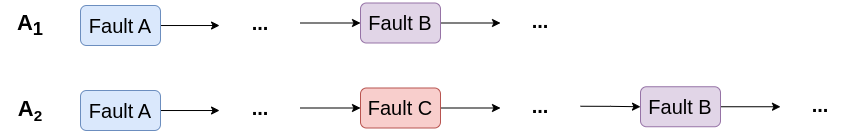
\includegraphics[scale=0.32]{img/red-subword.png}
        \end{figure}
        \vfill
    }

    \only<3>{
        \begin{itemize}
            \item[]
            \item \textbf{Redundancy} and \textbf{equivalence} aims to filter attacks for the user in multiple faults
            \item[]
        \end{itemize}
    
        \begin{definition}[Equivalence]
            An attack $a$ is \textbf{equivalent} to an attack $a'$ if their sequence of transitions are equal
        \end{definition}
    
        \begin{definition}[Fault-equivalence]
            An attack $a$ is \textbf{equivalent} to an attack $a'$ if their sequence of faulted transitions are equal
        \end{definition}
    
        \begin{figure}
            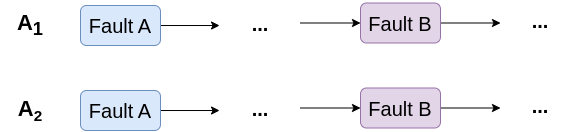
\includegraphics[scale=0.32]{img/red-min.drawio.png}
        \end{figure}
    }
\vfill
}
\end{frame}

\begin{frame}[fragile]{Experimentation}
\vfill
{\tiny
    \begin{columns}    
        \begin{column}{0.5\textwidth}
            Tested programs:
            \begin{itemize}
                \item \textit{Verify\_PIN} (\textbf{vp}): smart-card PIN verification process
                \item[] $\Rightarrow$ \textit{model}: test inversion
                \item \textit{RSA Cipher} (\textbf{rsa}): implementation of RSA encryption scheme. 
                \item[] $\Rightarrow$ \textit{model}: data load mutation
                \item \textit{Firmware Updater} (\textbf{fu}): updates a firmware from remote source
                \item[] $\Rightarrow$ \textit{models}: test inversion and data load mutation
            \end{itemize}
        \end{column}
        \begin{column}{0.5\textwidth}
            \onslide<2->{
                \begin{itemize}
                    \item Simplifies the number of attacks to consider
                    \item[] $\Rightarrow$ by a factor $200$ in a set of 15 examples from FISSC
                    \item[]
                    \item DSE is the main limit factor 
                    \item[] $\rightarrow$ with redundancy analysis matching on some examples
                \end{itemize}
            }    
        \end{column}
    \end{columns}

    \vspace{0.2cm}
    
    \onslide<2->{
        \begin{table}[p]            
            \caption{{\tiny Attack analysis on example programs}}\label{tbl:ch3:exp:fissc-results}
            \begin{center}
                \setlength\tabcolsep{4pt} % default value: 6pt
                \begin{tabular}{lll|lllll|lllll}
                \multicolumn{3}{l|}{Program} &  \multicolumn{5}{l|}{Attacks} & \multicolumn{5}{l}{Minimal attacks (with equivalence)}  \\
                Nom & LoCs & IPs &  1F & 2F & 3F & 4F & Total & 1F & 2F & 3F & 4F & Total \\
                \hline
                \hline
                vp0 & 25 & 4 &  12 & 21 & 18 & 7 & \textbf{58} & 3 & 0 & 0 & 0 & \textbf{3}  \\
                \hline
                vp4 & 45 & 11 &  34 & 118 & 180 & 147 & \textbf{479} & 3 & 0 & 1 & 0 & \textbf{4}  \\
                \hline
                vp7 & 78 & 8 &  4 & 36 & 116 & 173 & \textbf{329} & 1 & 2 & 0 & 0 & \textbf{3}  \\
                \hline
                rsa0 & 65 & 15 &  7 & 37 & 151 & 425 & \textbf{620} & 7 & 0 & 0 & 0 & \textbf{7}  \\
                \hline
                fu1 & 93 & 23  &  1 & 72 & 915 & 8191 & \textbf{9179} & 1 & 8 & 9 & 13 & \textbf{31}  \\
                \hline
                fu2  & 126 & 7  &  17 & 119 & 425 & 1031 & \textbf{1592} & 17 & 2 & 10 & 53 & \textbf{82}  \\
                \hline
                \hline
                \end{tabular}
            \end{center}
        \end{table} 
    }
}
\end{frame}


\begin{frame}[fragile]{Summary}
\vfill
{\small        
    My contributions:
    \begin{itemize}        
        \only<1>{
            \item \textbf{Python API :}
            \begin{itemize}
                \item \textbf{Manipulation of traces, analysis and models}
                \item \textbf{Fine fault space specification}
                \item \textbf{User accessibility: error handling, control on attack objective}
            \end{itemize}
        }
        \onslide<2->{
            \item Python API
            \begin{itemize}
                \item Manipulation of traces, analysis and models
                \item Fine fault space specification
                \item User accessibility: error handling, control on attack objective
            \end{itemize}
        }
        \only<2>{
            \item \textbf{Rewriting of Wolverine (mutation tool):}
            \begin{itemize}
                \item \textbf{Fault model combination}
                \item \textbf{Models data (+symbolic) and jump}
                \item \textbf{Automated countermeasures (TM, LM..)}
                \item \textbf{Switch to LLVM 9 (KLEE 2)}
            \end{itemize}
        }
        \onslide<3->{
            \item Rewriting of Wolverine (mutation tool):
            \begin{itemize}
                \item Fault model combination
                \item Models data (+symbolic) and jump
                \item Automated countermeasures (TM, LM..)
                \item Switch to LLVM 9 (KLEE 2)
            \end{itemize}
        }   
        \only<3>{      
            \item \textbf{Analysis:}
            \begin{itemize}
                \item \textbf{Redundancy / Equivalence}
                \item \textbf{Hotspots analysis}
                \item \textbf{Countermeasure analysis}
            \end{itemize}
        }
        \onslide<4->{
            \item Analysis:
            \begin{itemize}
                \item Redundancy / Equivalence
                \item Hotspots analysis
                \item Countermeasure analysis
            \end{itemize}
        }
        \onslide<4->{
            \item \textbf{Combination of Lazart with static analysis (Frama-C) on Wookey boot loader [Lacombe 2023]}
            \item \textbf{Filed at APP}
        }
    \end{itemize}
}        
\vfill
\end{frame}


\section{Countermeasures placement}

\subsection{Introduction}

\begin{frame}[fragile]{Placement of software countermeasures}
    \begin{columns}
        \begin{column}{0.55\textwidth}    
            \lstset{style=customc, escapeinside={(*}{*)}}
            \begin{lstlisting}
bool compare(uchar* a1, uchar* a2, size_t size)
{
    bool ret = true;
    size_t i = 0; 
    for(; i < size; i++) {
        
        if(a1[i] != a2[i]) {
            ret = false;
        }
    }
        
    return ret;
}
            \end{lstlisting}	
            \vfill
        \end{column}
        \begin{column}{0.55\textwidth}
            \begin{small}
                \begin{itemize}
                    \item \textbf{Goal}: help to place countermeasures in multiple fault context (P2 and P3)
                    \item[] $\rightarrow$ several fault models can be considered
                    \item[] $\rightarrow$ countermeasures can be attacked with each fault model
                    \item[] $\rightarrow$ countermeasures can introduce attacks
                    \item[] $\rightarrow$ using a defined attack objective
                \end{itemize}
            \end{small}
        \vfill
        \end{column}
    \end{columns}
\end{frame}

\begin{frame}[fragile, noframenumbering]{Placement of software countermeasures}
    \begin{columns}
        \begin{column}{0.55\textwidth}
            \lstset{style=customc, escapeinside={(*}{*)}}
            \begin{lstlisting}
bool compare(uchar* a1, uchar* a2, size_t size)
{
    bool ret = true;
    size_t i = 0; 
    for(; i < size; i++) {
        (*{\color{mauve} if(i >= size) killcard();}*) // Duplication (true)
        (*{\color{mauve} if(i >= size) killcard();}*) // Triplication (true)

        (*{\color{mauve} uchar a1\_dup = a1[i]; }*) // Load duplication
        (*{\color{mauve} if(a1\_dup != a1[i]) killcard(); }*)
        (*{\color{mauve} uchar a2\_dup = a2[i]; }*) // Load duplication
        (*{\color{mauve} if(a1\_dup != a1[i]) killcard(); }*) 
        
        if(a1[i] != a2[i]) {
            (*{\color{mauve} if(i >= size) killcard();}*) // Duplication (true)
            (*{\color{mauve} if(i >= size) killcard();}*) // Triplication (true)
            ret = false;
        }
    }
    (*{\color{mauve} if(i != size) killcard();}*) // Duplication (false)
    (*{\color{mauve} if(i != size) killcard();}*) // Triplication (false)
        
    return ret;
}
            \end{lstlisting}	
            \vfill
        \end{column}
        \begin{column}{0.55\textwidth}
    	   \begin{small}
                 \begin{itemize}
                     \item \textbf{Goal}: help to place countermeasures in multiple fault context (P2 and P3)
                     \item[] $\rightarrow$ several fault models can be considered
                     \item[] $\rightarrow$ countermeasures can be attacked with each fault model
                     \item[] $\rightarrow$ countermeasures can introduce attacks
                     \item[] $\rightarrow$ using a defined attack objective
                 \end{itemize}
    	   \end{small}
            \vfill
        \end{column}
    \end{columns}
\end{frame}

\begin{frame}[fragile]{Placement of software countermeasures} 
    \textbf{Goal}: help to place countermeasures in multiple fault context 
    
    \begin{itemize}
        \item Target robustness in $N$ faults
        \item Give guarantees even if trace exploration is not complete
        \item Using a catalog of countermeasures schemes with \textit{Injection Point} (IP) granularity 
        \item []
    \end{itemize}

    \textbf{Approach:}
    \begin{itemize}
        \item  Compositional analysis using:
        \begin{itemize}
            \item  \textit{Isolation analysis} of countermeasures schemes
            \item[] $\rightarrow$ Notion of protection coefficient
            \item Exploration of attacks traces on the program P
        \end{itemize}        
        \item Placement algorithms
    \end{itemize}
\vfill
\end{frame}

\subsection{Analysis in isolation}

\begin{frame}[fragile]{Principle of analysis in isolation}
    \begin{columns}
        \begin{column}{0.2\textwidth}
            \begin{figure}
                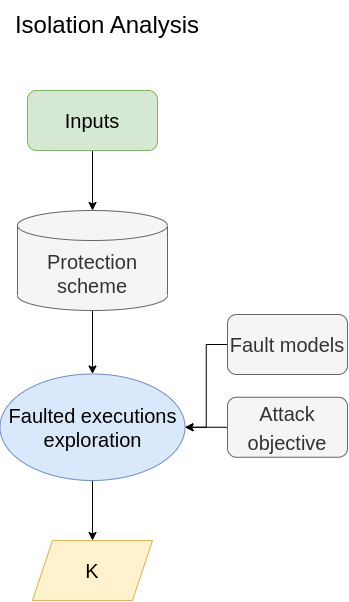
\includegraphics[scale=0.25]{img/out-of-context-metho.png}
            \end{figure}
    	\vfill
        \end{column}
        \begin{column}{0.04\textwidth} \end{column}
        \begin{small}
            \begin{column}{0.75\textwidth}
                \begin{itemize}
                    \item Analysis of countermeasures scheme in isolation
                    \item Focus on countermeasures with IP granularity
                    \item[] $\rightarrow$ A \textbf{protection scheme} describe how an IP is protected
                    \item Research of the \textit{protection coefficient} (K) of the protection scheme:
                    \item[] $\rightarrow$ e.g. \textit{How many faults are required to induce an abnormal behavior (not detected) for the protected IP ?}
                    \item[] $\rightarrow$ Unprotected IP has a $K = 1$
                    \item[] $\rightarrow$ Can be computed with Lazart 
                \end{itemize}
            \end{column}             
        \end{small}
    \end{columns}
\end{frame}

\begin{frame}[fragile]{Analysis in isolation of Branch duplication scheme}
    \begin{columns}
        \begin{column}{0.25\textwidth}
            \begin{figure}
                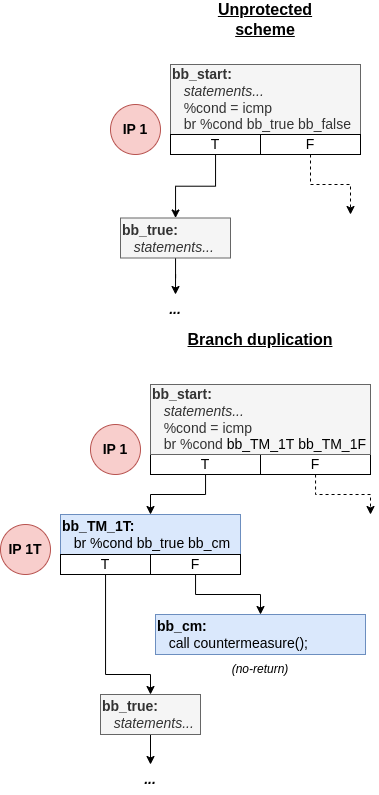
\includegraphics[scale=0.25]{img/branch-mul.png}
            \end{figure}
            \vfill
        \end{column}
        \begin{column}{0.04\textwidth} \end{column}
        \begin{small}
            \begin{column}{0.7\textwidth}
                Branch Multiplication ($BM_n$): n-plication of a conditional branch
                \vspace{0.3cm}
                
                Isolation analysis with \textit{Branch Inversion} fault model                
                \vspace{0.3cm}
                
                \onslide<2-> {
                    Need to define:
                    \begin{itemize}
                        \item Input(s) of the scheme
                        \onslide<3->{$\rightarrow$ \textbf{the \texttt{\%cond} temporary}}
                        \item Output(s) of the scheme \onslide<3->{$\rightarrow$ \textbf{the destination branch}}
                        \item Entry point(s) \onslide<4->{$\rightarrow$ \textbf{the \texttt{br} instruction (\texttt{bb\_start})}}
                        \item Output point(s) \onslide<4->{$\rightarrow$ \textbf{the destination block (\texttt{bb\_true})}}
                        \item Attack surface \onslide<5->{$\rightarrow$ \textbf{$IP\; 1$ and $IP\; 1T$ with BI fault model}}
                        \item Nominal behavior \onslide<6->{$\rightarrow$ \textbf{reach \texttt{bb\_true} if and only if \%cond is true}}
                    \end{itemize}
                }
            \end{column}
        \end{small}
    \end{columns}
\end{frame}

\begin{frame}[fragile]{Analysis in isolation of BM schemes}
    \begin{columns}
        \begin{column}{0.45\textwidth}
            \begin{figure}
                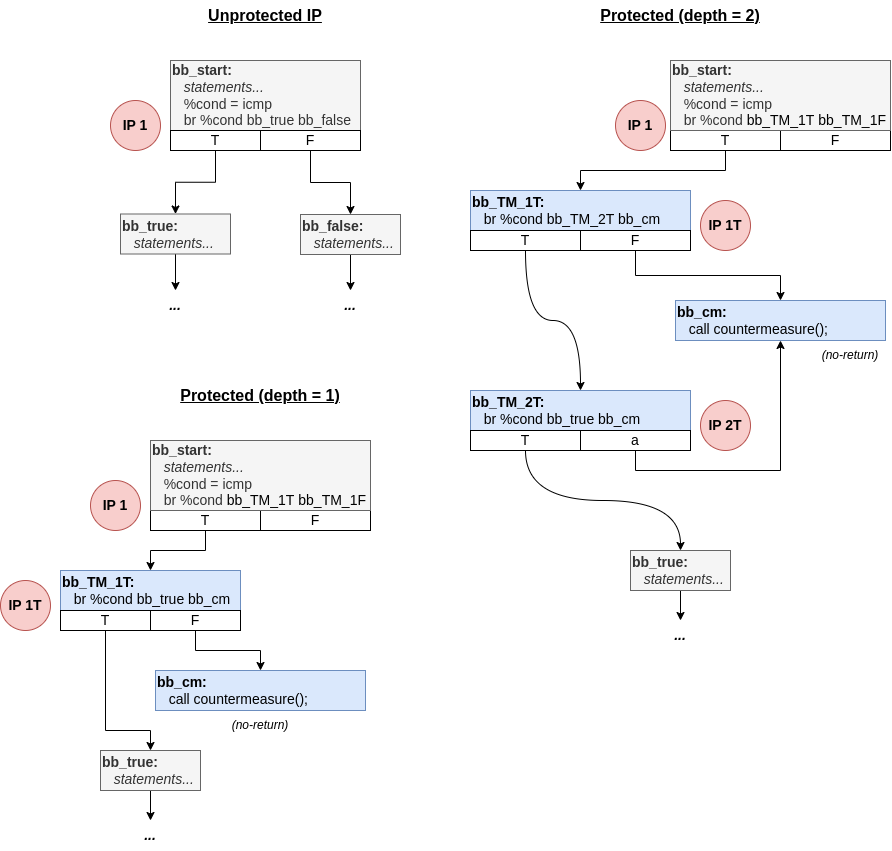
\includegraphics[scale=0.20]{img/cm-mul-test-large.png}
            \end{figure}
            \vfill
        \end{column}
        \begin{column}{0.07\textwidth} \end{column}
        \begin{small}
            \begin{column}{0.48\textwidth}
                \textbf{Branch Multiplication} ($BM_n$): n-plication of a conditional branch                
                \vspace{0.3cm}
                
                Isolation analysis with \textit{Branch Inversion} fault model
                \vspace{0.3cm}
        
                \begin{table}[ht]
                    \begin{tiny}
                        \begin{center}
                            \setlength\tabcolsep{2.1pt} % default value: 6pt
                            \begin{tabular}{l|ccccc}
                                Countermeasure & 0-faults & 1-fault & 2-faults & 3-faults  & \textbf{$K$} \\
                                \hline
                                $BM_0$ & 0 & 1 & 0 & 0 & \textbf{1}\\
                                $BM_1$ & 0 & 0 & 1 & 0 & \textbf{2} \\
                                $BM_2$ & 0 & 0 & 0 & 1 & \textbf{3}
                            \end{tabular}
                        \end{center}                         
                    \end{tiny}
                    \caption{$BM$ isolation analysis}
                \end{table}
            \end{column}
        \end{small}
    \end{columns}
\end{frame}

\begin{frame}[fragile]{Analysis in isolation of LM schemes}
    \begin{columns}
        \begin{column}{0.35\textwidth}
            \begin{figure}
                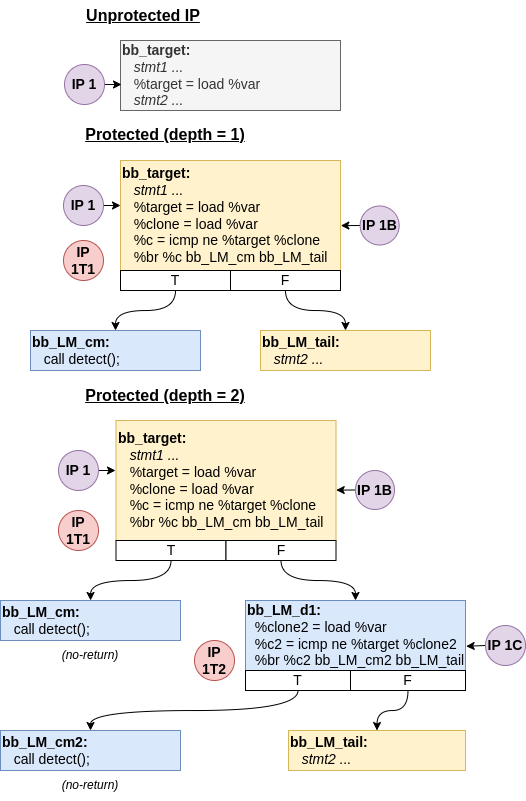
\includegraphics[scale=0.24]{img/cm-mul-load-full-sepend.drawio.png}
            \end{figure}
            \vfill
        \end{column}
        \begin{column}{0.01\textwidth} \end{column}
        \begin{small}
            \begin{column}{0.65\textwidth}            
                \textbf{Load Multiplication} ($LM_n$): n-plication of a \texttt{load} instruction (and checks)
                    
                \begin{itemize}
                    \item []
                \end{itemize}
                
                Isolation analysis with \textit{Data Load} and \textit{Branch Inversion} fault models
                \vspace{0.2cm}
                
                \begin{itemize}
                    \item Input: the value stored in \texttt{\%var} memory cell
                    \item Output: the value loaded in \texttt{\%target}
                    \item Nominal behavior: \texttt{\%target} stores \texttt{\%var}'s value
                \end{itemize}
                
                \begin{table}[ht]
                    \begin{tiny}
                        \begin{center}
                            \setlength\tabcolsep{2.1pt}
                            \begin{tabular}{l|ccccc}
                                Countermeasure & 0-faults & 1-fault & 2-faults & 3-faults &  \textbf{$K$} \\
                                \hline
                                $LM_0$ & 0 & 1 & 0 & 0 &  \textbf{1}\\
                                $LM_1$ & 0 & 0 & 1 & 0 &  \textbf{2} \\
                                $LM_2$ & 0 & 0 & 0 & 1 &  \textbf{3}
                            \end{tabular}
                        \end{center} 
                    \end{tiny}
                    \caption{$LM$ isolation analysis}
                \end{table}
            \end{column}
        \end{small}
    \end{columns}
\end{frame}

\subsection{Placement algorithms}

\begin{frame}[fragile]{Placement algorithms principles}
	\begin{small}
        \textbf{GOAL:} generate a P' program which is robust to $N$ faults
        \vspace{0.25cm}
        
        $\Rightarrow$ Give guarantees that P' is \textit{more robust than P} even if trace set is \textit{incomplete} or if catalog is incomplete
        \vspace{0.45cm}
        
        \onslide<2->{
            Basic structure of placement algorithms:
            \begin{enumerate}
                \item Obtain set of attack traces
                \item[] $\Rightarrow$ Computed with all fault models and the user-defined attack objectives
                \item Compute \textbf{required protection coefficient} ($K_{ip}$) for each IP (initialized to 1)
                \item Generate $P'$ with protection scheme matching the \textbf{required protection coefficients}
                \item[] $\Rightarrow$ Using a catalog $\mathcal{C}$ of countermeasures (with computed $K_{ip}$)
            \end{enumerate}        
        \vspace{0.5cm}
        }
        \onslide<3>{
            Three approaches:
            \begin{itemize}
                \item \textit{Systematic} placement: protect all IPs of a set with K > N
                \item \textit{Block} placement: protect at least one IPs of all attacks with K > N
                \item \textit{Distributed} placement: protect IPs such as for each trace, the sum of K of each IP is greater than N
            \end{itemize}
        }        
        \vfill
	\end{small}
\end{frame}

\begin{frame}[fragile]{Systematic placement algorithms}
    \begin{columns}
        \begin{column}{0.5\textwidth}
            \begin{tiny}
                \lstset{style=custompython}
                \begin{lstlisting}
def placement_min(C: Catalog, P: Program, M: AttackModel, n: int):
    # Get sucessfull non-detected attacks.
    attacks = T_s(P, M, n)
    # Filter with minimals attacks.
    minimals = RedundacyAnalysis(attacks).minimals()
    
    # Initial protection factors Kn at 1 for all IP.
    required_kn = { IPA: 1, IPB: 1, ..., IPN: 1 }

    # Apply ponderation of n for all IP in traces
    for attack in minimals:
        for IP in attack:
            required_kn[IP] = n + 1 # Make IP robust en n faults.

    # Generation of P'
    P` = P
    for IP, kn in required_kn:
        S = C.get_cm(IP.model(), kn) # Select protection scheme from catalog
        P` = S(P`, IP) # Apply local protection        
    return P`    \end{lstlisting}
            \end{tiny}
        \end{column}
        \begin{column}{0.5\textwidth}
            \begin{tiny}
                \textbf{Systematic algorithms:}
                \begin{itemize}
                    \item Naive placement (\texttt{naive}): protect all IP with K > N
                    \item [] $\rightarrow$ \textit{corresponds to standards systematic protection tools}% \cite{ Lalande/ESORICS14, Ferriere/LLVM19}}
                    \item [] $\rightarrow$ do not require attacks paths
                    \item Attack placement (\texttt{atk}): protect all IP in attacks with K > N
                    \item Minimal placement  (\texttt{min}) (\textbf{on left)}: protect all IP in minimal attacks with K > N
                \end{itemize}
                
                \vspace{0.6cm}
                \onslide<2-> {
                    Guarantees:
                    \begin{itemize}
                        \item \textbf{Robust in $N$ faults} if the catalog provides required $K$ for each IP (complete catalog) and if the entry trace set is complete
                        \onslide<3->{\item \textbf{At least as robust as $P$} otherwise}
                        \onslide<3->{\item[] $\rightarrow$ if the catalog is incomplete, \textit{vulnerable traces in $P'$ are known}}
                    \end{itemize}
                }
                \vfill
            \end{tiny}
        \end{column}
    \end{columns}
\end{frame}

\begin{frame}[fragile]{Block placement algorithm}
    \begin{columns}
        \begin{column}{0.5\textwidth}
            \begin{tiny}
                \lstset{style=custompython}
                \begin{lstlisting}
def placement_bloc_h(C: Catalog, P: Program, M: AttackModel, n: int):
    # Get sucessfull non-detected attacks.
    attacks = T_s(P, M, n)
    # Filter with minimals attacks.
    minimals = RedundacyAnalysis(attacks).minimals()
    
    # Initial protection factors Kn at 1 for all IP.
    required_kn = { IPA: 1, IPB: 1, ..., IPN: 1 }
            
    # For all attacks by faults count.
    for order in 1 to n:
        # Loop trought order-faults attacks by number of associated redundant attacks.
        for attack in minimals.where(order=order).sort_by(Minimals):
            if is_protected(attack, required_kn):
                continue
            # Make attack robust in n faults
            IP = select IP in attack with most occurence
            required_kn[IP] = n + 1

    # Generation of P'
    P` = P
    for IP, kn in required_kn:
        S = C.get_cm(IP.model(), kn) # Select protection scheme from catalog
        P` = S(P`, IP) # Apply local protection        
    return P`   \end{lstlisting}
            \end{tiny}
        \end{column}
        \begin{column}{0.5\textwidth}
        	\begin{tiny}
                Protection of at least one IP per minimal attack with K > N
                \begin{itemize}
                    \item [] $\rightarrow$ heuristic based
                \end{itemize}
                \vspace{0.6cm}
                
                Guarantees:
                \begin{itemize}
                    \item \textbf{Robust in $N$ faults} if the catalog provides required $K$ for each IP (complete catalog) and if the entry trace set is complete
                    \item \textbf{At least as robust as $P$} otherwise
                    \item[] $\rightarrow$ if the catalog is incomplete, \textit{vulnerable traces in $P'$ are known}
                \end{itemize}
                \vspace{1cm}
                \textit{How to be sure than no attack paths is introduced by non-protected IPs ?}
                
                \vfill
        	\end{tiny}
        \end{column}
    \end{columns}
\end{frame}

\begin{frame}[fragile]{Compositional analysis placement}
    \begin{columns}
        \begin{column}{0.6\textwidth}
            \begin{figure}
                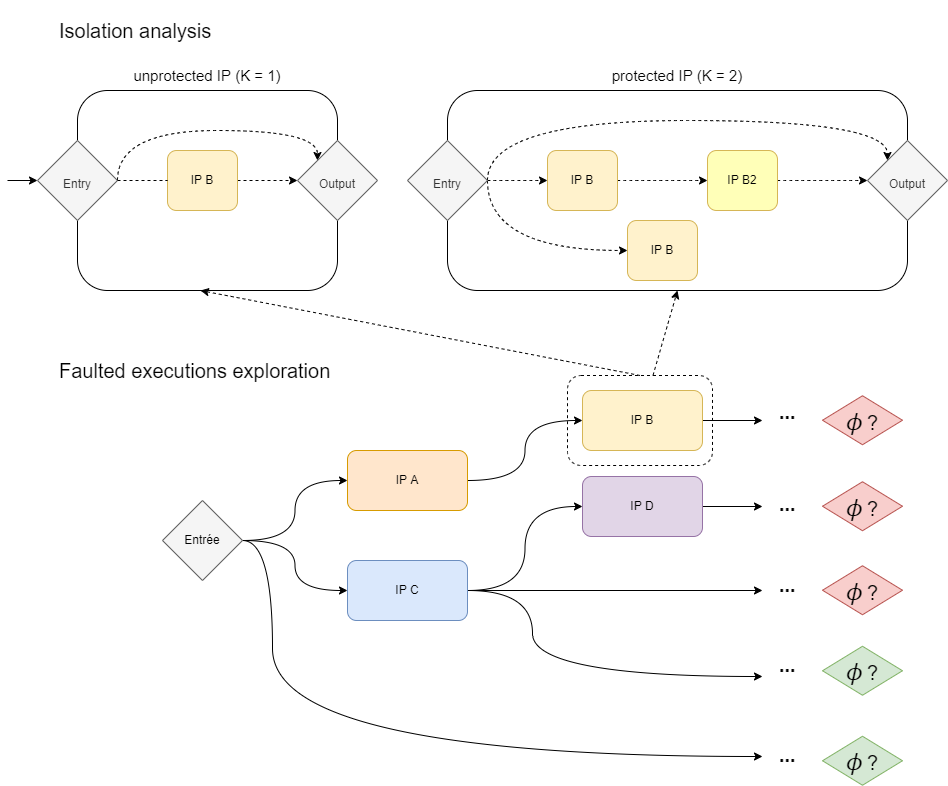
\includegraphics[scale=0.21]{img/placement-isolation-end.drawio.png}
            \end{figure}
        \end{column}
        \begin{column}{0.4\textwidth}
            \begin{tiny}
                \begin{itemize}
                    \item Isolation analysis for each considered protection scheme with all studied fault models                
                    \item []
                    \item []
                    \item []
                    \item []                
                    \item Attacks traces gives guarantees on which IP violation can lead to an attack
                    \item [] $\rightarrow$ \textit{Here, $IP A$ can be left unprotected if $IP B$ is protected}
                    \item []
                \end{itemize}
    
                \onslide<2>{
                    $\Rightarrow$ \textbf{Protection can be distributed between the IPs }
                }
            \end{tiny}
        \end{column}
\end{columns}
\end{frame}

\begin{frame}[fragile]{Optimal distributed placement} 
    \begin{tiny}
        \begin{itemize}
            \item  Distribute protections of IPs inside minimal attacks traces to ensure at least N + 1 faults are required to obtain attacks
            \item[] $\rightarrow$ usable if the catalog $\mathcal{C}$ does not contains CM for K > N
            \item[]
            \item An Integer Linear Programming (ILP) optimization problem 
            \item[] $\rightarrow$ attacks gives constraints on the protection to apply
        \end{itemize}
        
        \begin{figure}
            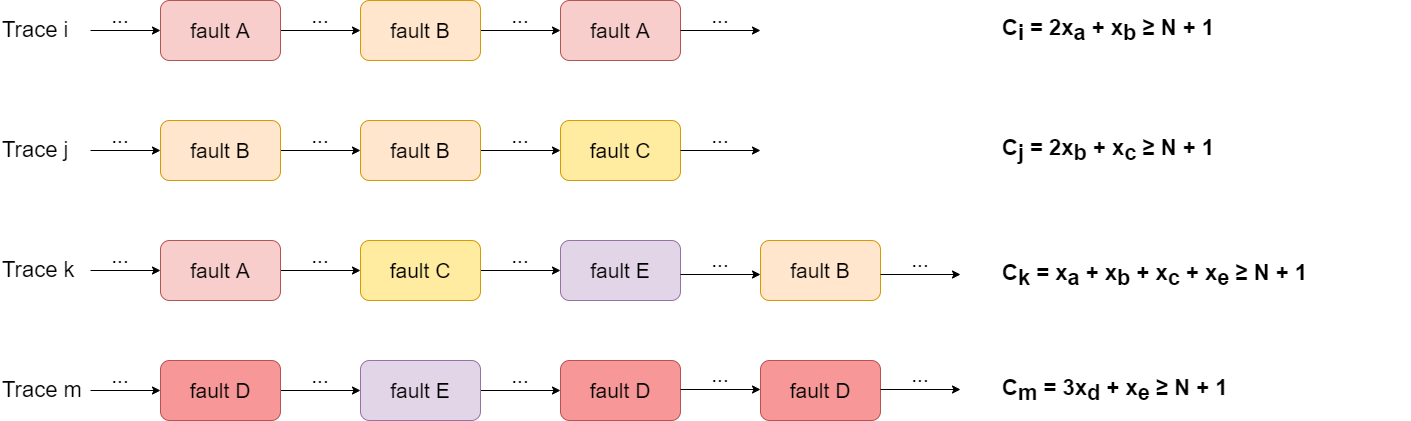
\includegraphics[scale=0.18]{img/placement-eq.drawio.png}
        \end{figure}
        
        \begin{itemize}
            \item[]
            \item[] Research of the \textbf{optimal} placement
            \item[] $\Rightarrow$ minimize the protection weight $Z = x_a + x_b + ... + x_p$
            \item[]
            \item require to ensure that all states produced by the protected IPs are studied in trace exploration fault models 
            \item[] $\rightarrow$ \textit{guarantees on partially protected IPs}
        \end{itemize}
    \end{tiny}
\end{frame}

\begin{frame}[fragile]{Optimal distributed placement}
    \begin{columns}
        \begin{column}{0.5\textwidth}
            \begin{tiny}
                \lstset{style=custompython}
                \begin{lstlisting}
def placement_rep_opt(C: Catalog, P: Program, M: AttackModel, n: int):
    # Get sucessfull non-detected attacks.
    attacks = T_s(P, M, n)
    # Filter with minimals attacks.
    minimals = RedundacyAnalysis(attacks).minimals()
    
    # Initial protection factors Kn at 1 for all IP.
    required_kn = { IPA: 1, IPB: 1, ..., IPN: 1 }
    
    constraints = [] # constraints for ILP
    for attack in minimals:
        constraints += compute_constraint(attack)
    
    required_kn = solve_ilp(constraints, required_kn)
    
    # Generation of P'
    P` = P
    for IP, kn in required_kn:
        S = C.get_cm(IP.model(), kn) # Select protection scheme from catalog
        P` = S(P`, IP) # Apply local protection        
    return P`   \end{lstlisting}
            \end{tiny}
        \end{column}
        \begin{column}{0.5\textwidth}
            \begin{tiny}
                Optimal placement using ILP problem encoding:
                \begin{enumerate}
                    \item Encode constraints from attack traces (lines 10-12)
                    \item Solve ILP (line 14)
                    \item Generate P' (lines 17-20)
                \end{enumerate}
    
                \vspace{0.6cm}
                Guarantees:
                \begin{itemize}
                    \item \textbf{Robust in $N$ faults} if the catalog provides required $K$ for each IP (complete catalog) and if the entry trace set is complete
                    \item[] $\rightarrow$ and \textbf{optimal} (i.e. minimal set of protections wrt $\mathcal{C}$) 
                    \item \textbf{At least as robust as $P$} otherwise
                    \item[] $\rightarrow$ if the catalog is incomplete, \textit{vulnerable traces in $P'$ are known}
                \end{itemize}        
                \vfill
            \end{tiny}
        \end{column}
    \end{columns}
\end{frame}

\subsection{Experimentation}

\begin{frame}{Experimentation - verify\_pin} 
    \begin{small}
        \textit{verify\_pin} \cite{Dureuil/PPLCC16} (\textbf{VP}): smart-card PIN verification process
        
        \begin{itemize}
             \item \textit{fault model:} branch inversion
             \item \textit{inputs:} input PINs are different and symbolic
             \item \textit{attack objective:} being authenticated or do not decrement the try counter 
             \item \textit{countermeasures:}
             \begin{itemize}
                 \item \textit{integrated:} hardened boolean, fixed time loop
                 \item \textit{placement:} branch multiplication (BM)
             \end{itemize}
        \end{itemize}
    \end{small}
    
    \begin{table}[htp]
        \begin{tiny}
            \begin{center}
                \begin{tabular}{lll|l|llll|l}
                \multicolumn{3}{c}{Exp.} & \multicolumn{1}{c}{Algo.} & \multicolumn{4}{c}{$\sum$ of protections} & \multicolumn{1}{c}{Robust} \\
                \hline
                Program & Fault Model & IPs &  & 1-fault & 2-faults & 3-faults & 4-faults &  \\
                \hline
                \hline
                \texttt{vp2b} & BI & \multicolumn{1}{r|}{8} & naive & 8 & 16 & 24 & 32 & \checkmark \\
                 &  &  & atk & \textbf{3} & 8 & 12 & 16 & \checkmark \\
                 &  &  & min & \textbf{3} & 8 & 12 & 16 & \checkmark \\
                 &  &  & block & \textbf{3} & \textbf{6} & \textbf{9} & \textbf{12} & \checkmark \\
                 &  &  & opt & \textbf{3} & \textbf{6} & \textbf{9} & \textbf{12} & \checkmark
                \end{tabular}
            \end{center}
        \end{tiny}
    \end{table}
\vfill
\end{frame}

\begin{frame}{Experimentations - FU1} 
    \begin{small}
        \textit{firmware\_updater} v1 (\textbf{fu1}): updates a firmware from remote source
        \begin{itemize}
            \item \textit{fault model:} branch inversion + data load
            \item \textit{inputs:} input PINs are different and symbolic
            \item \textit{attack objective:} load a corrupted firmware or avoid load
            \item \textit{countermeasures:}
            \begin{itemize}
                \item \textit{integrated:} systematic tests duplication
                \item \textit{placement:} branch multiplication (BM) and load multiplication (LM)
            \end{itemize}
        \end{itemize}
    \end{small}
    
    \begin{table}[htp]
        \begin{tiny}
            \begin{center}
            \begin{tabular}{lll|l|llll|l}
                \multicolumn{3}{c}{Exp.} & \multicolumn{1}{c}{Algo.} & \multicolumn{4}{c}{$\sum$ of protections} & \multicolumn{1}{c}{Robust} \\
                \hline
                Program & Fault Model & IPs &  & 1-fault & 2-faults & 3-faults & 4-faults &  \\
                \hline
                \hline
                \texttt{fu1} & BI & \multicolumn{1}{r|}{42} & naive & 42 & 84 & 126 & 168 & \checkmark \\
                &  &  & atk & \textbf{0} & 28 & 42 & 88 & \checkmark \\
                &  &  & min & \textbf{0} & 28 & 42 & 72 & \checkmark \\
                &  &  & block & \textbf{0} & 14 & 21 & 28 & \checkmark \\
                &  &  & opt & \textbf{0} & \textbf{7} & \textbf{14} & \textbf{21} & \checkmark \\
                \hline
                & DL & \multicolumn{1}{r|}{2} & naive & 2 & 4 & 6 & 8 & \checkmark \\
                &  &  & atk & 1 & 4 & 6 & 8 & \checkmark \\
                &  &  & min & \textbf{1} & \textbf{2} & \textbf{3} & \textbf{4} & \checkmark \\
                &  &  & block & \textbf{1} & \textbf{2} & \textbf{3} & \textbf{4} & \checkmark \\
                &  &  & opt & \textbf{1} & \textbf{2} & \textbf{3} & \textbf{4} & \checkmark \\
                \hline
                & BI+DL & \multicolumn{1}{r|}{44} & naive & 44 & 88 & 132 & 176 & \checkmark \\
                &  &  & atk & \textbf{1} & 32 & 60 & 96 & \checkmark \\
                &  &  & min & \textbf{1} & 32 & 60 & 80 & \checkmark \\
                &  &  & block & \textbf{1} & 16 & 24 & 32 & \checkmark \\
                &  &  & opt & \textbf{1} & \textbf{9} & \textbf{17} & \textbf{25} & \checkmark \\
            \end{tabular}
            \end{center}
        \end{tiny}
    \end{table}
\vfill
\end{frame}

\subsection{Summary}

\begin{frame}{Summary} 
    \begin{small}
        \begin{itemize}
            \item Robustness of placement depend on the property of the catalog $\mathcal{C}$
            \item[]
            \item P' is guaranteed to be robust for N faults if the required protection coefficients (K) are available
            \item[] $\rightarrow$ if not, attack traces on P' are known
            \item []$\rightarrow$ more robust than P even if trace set is incomplete
            \item[]
            \item Protection weight: $distributed \leq block \leq min \leq atk \leq naive$ 
            \item[] $\rightarrow$ Optimal placement is guaranteed with ILP
            \item[]
        \end{itemize}

        \begin{table}[h]
            \begin{tiny}
                \begin{center}
                    \begin{tabular}{l|l|ll|l|lll}
                        Algorithme & Type & \multicolumn{2}{l|}{Guarantees $P'$} & Complexity & \multicolumn{3}{l}{Required analysis} \\
                         &  & Robust & Optimal &  & AA & Red & HS \\
                         \hline
                        naive & syst. & \checkmark & - & $O(t)$ & \checkmark & - & - \\
                        atk & syst. & \checkmark & - & $O(t)$ & \checkmark & - & - \\
                        min & syst. & \checkmark & - & $O(t)$ & \checkmark & \checkmark & - \\
                        block & block & \checkmark & - & $O(t)$ & \checkmark & \checkmark & \checkmark \\
                        opt & distributed & \checkmark & \checkmark & NP-Complete & \checkmark & \checkmark & - \\
                    \end{tabular}
                \end{center} 
            \end{tiny} 
        \end{table}
        
        \begin{itemize}
            \item[]
            \item Placement algorithm is fast compared to trace generation (DSE)
            \item[] $\rightarrow$ even with optimal algorithm and ILP (1-fault attacks)
        \end{itemize}
    \end{small}
\vfill
\end{frame}


\section{Countermeasures optimization}

\subsection{Problematic}

\begin{frame}[fragile]{Countermeasures optimization approach} 
    \begin{small}
        \begin{itemize}
        \item Can some part of the countermeasure be removed without adding new attacks ?  
        \item[] $\Rightarrow$ Probl. P2 \& P4
        \item[] 
        \end{itemize}
        
        \onslide<1->{
            \begin{figure}[!ht]
            \centering
                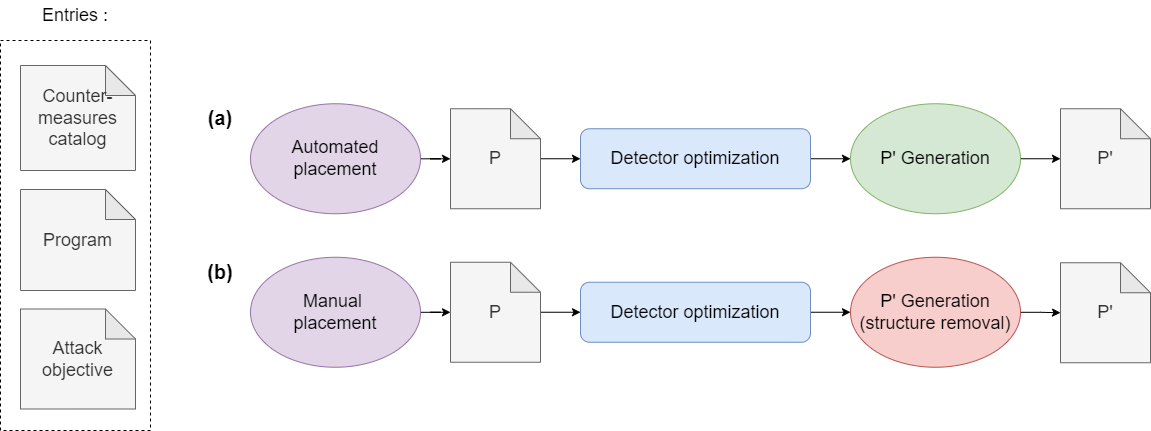
\includegraphics[scale=0.19]{img/placement-ccpo2-en.drawio.png}
                \label{fig:ccpo-metho}
            \end{figure}
        }
        
        \onslide<2->{
            \begin{itemize}
            \item[]
            \item \textbf{Approach:}
            \item[] $\Rightarrow$ focus on the subclass of detector-based countermeasures
            \item[] $\Rightarrow$ based on the execution with non-blocking detectors
            \end{itemize}
        }
    \end{small}
    \vfill
\end{frame}

\begin{frame}[fragile]{Definitions - Detectors and bodies} 
    \begin{small}
        \begin{columns}
            \begin{column}{0.5\textwidth}
                \begin{tiny}  
                    We divide a \textbf{detector-based countermeasure} in two parts:
                    \vspace{0.25cm}
                    
                    \begin{itemize}
                        \item {\color{RedViolet}Detectors} are control point in the program corresponding to sanity checks about the current state
                        \item The {\color{Bittersweet}countermeasure's bodies}: shadow variables, parameters, additional computation etc.
                    \end{itemize}
                    \vspace{0.2cm}
                    
                    \onslide<2->{
                         Examples
                         \begin{itemize}
                             \item \textit{Test duplication} (\textbf{TD}) 
                             \item \textit{Load Multiplication} (\textbf{LM})
                             \item \textit{SecSwift Control Flow} (\textbf{SSCF})\cite{Ferriere/LLVM19}: associates an unique identifier to each basic block and uses a xor-based mechanism to ensure that the correct branch has been taken
                             \item \textbf{LBH} \cite{Lalande/ESORICS14}: introduce step counters to protect against C-level instruction skips. Each counter verification is a \texttt{detector}
                         \end{itemize}
                    }
                \end{tiny}
            \end{column}
            \begin{column}{0.5\textwidth}
                \lstset{escapeinside={<@}{@>}}
                \lstset{style=customc}
                \begin{lstlisting}
bool compare(uchar* a1, uchar* a2,
    size_t size<@{\color{Bittersweet}, size\_t size\_dup}@>) {
    size_t i = 0u;
    bool result = true;
    <@{\color{Bittersweet}bool result\_dup = true;}@>
    
    for(; i < size; i++) {
        if(a1[i] != a2[i])
            result = false;
        <@{\color{Bittersweet}if(a1[i] != a2[i])}@>
            <@{\color{Bittersweet}result\_dup = false;}@> 
        
        <@{\color{RedViolet}if(result != result\_dup)}@>
            <@{\color{RedViolet}countermeasure();}@>
    }

    <@{\color{RedViolet}if(i != size)}@>
        <@{\color{RedViolet}countermeasure();}@>
    <@{\color{RedViolet}if(i != size\_dup)}@>
        <@{\color{RedViolet}countermeasure();}@>

    return result;
}
                \end{lstlisting}
            \end{column}
        \end{columns}
        \vspace{0.1cm}
    
        \textbf{Objectives}: 
        \begin{itemize}
            \item determine if some {\color{RedViolet}detector} could be removed, without adding any attack paths for the considered attack model.
        \end{itemize}
    \end{small}
\end{frame}


\subsection{Methodology}

\begin{frame}[fragile]{Countermeasure optimization - Idea: don't stop execution after detection } 
    \begin{tiny}
        \begin{itemize}
            \item Detector are considered as a structure \texttt{if(cond) killcard();} that can be attacked and \texttt{killcard} an atomic detection function
        \end{itemize}
        \onslide<2->{
            \begin{itemize}
                \item \textit{Intuition:} Explore the program executions by noting at each detector location if the corresponding detector would be triggered 
                \item[] $\Rightarrow$ all variation of detectors are considered in one single exploration.
                \item [] $\Rightarrow$ require side-effect free property on detectors
            \end{itemize}
        }
        \only<1>{
                \begin{figure}
                    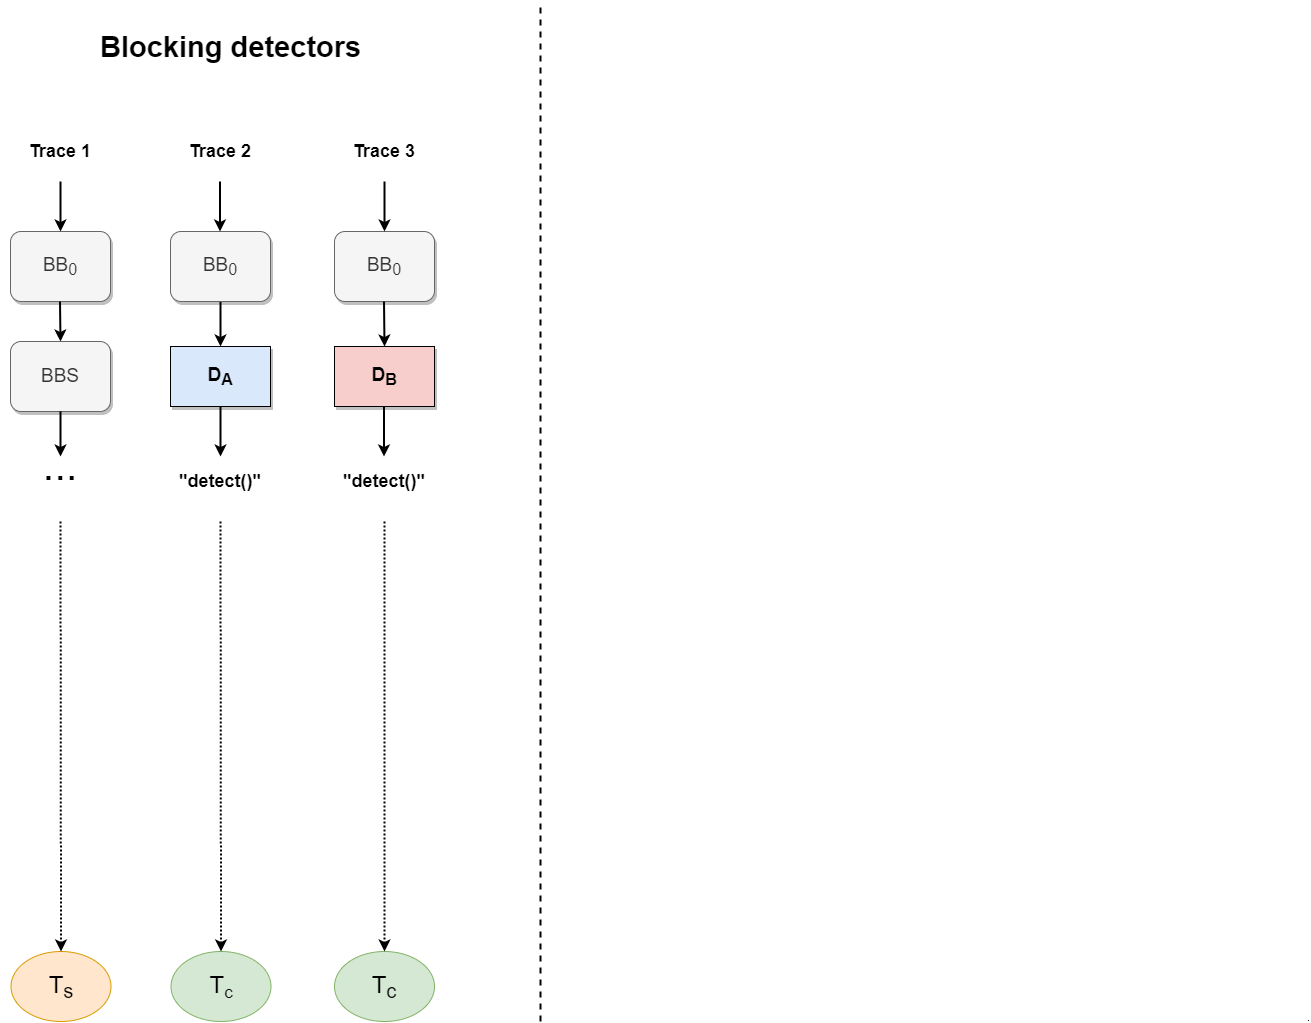
\includegraphics[scale=0.187]{img/CCP-prop-stopping2-simple.png}
                \end{figure}
        }
        \only<2>{
                \begin{figure}
                    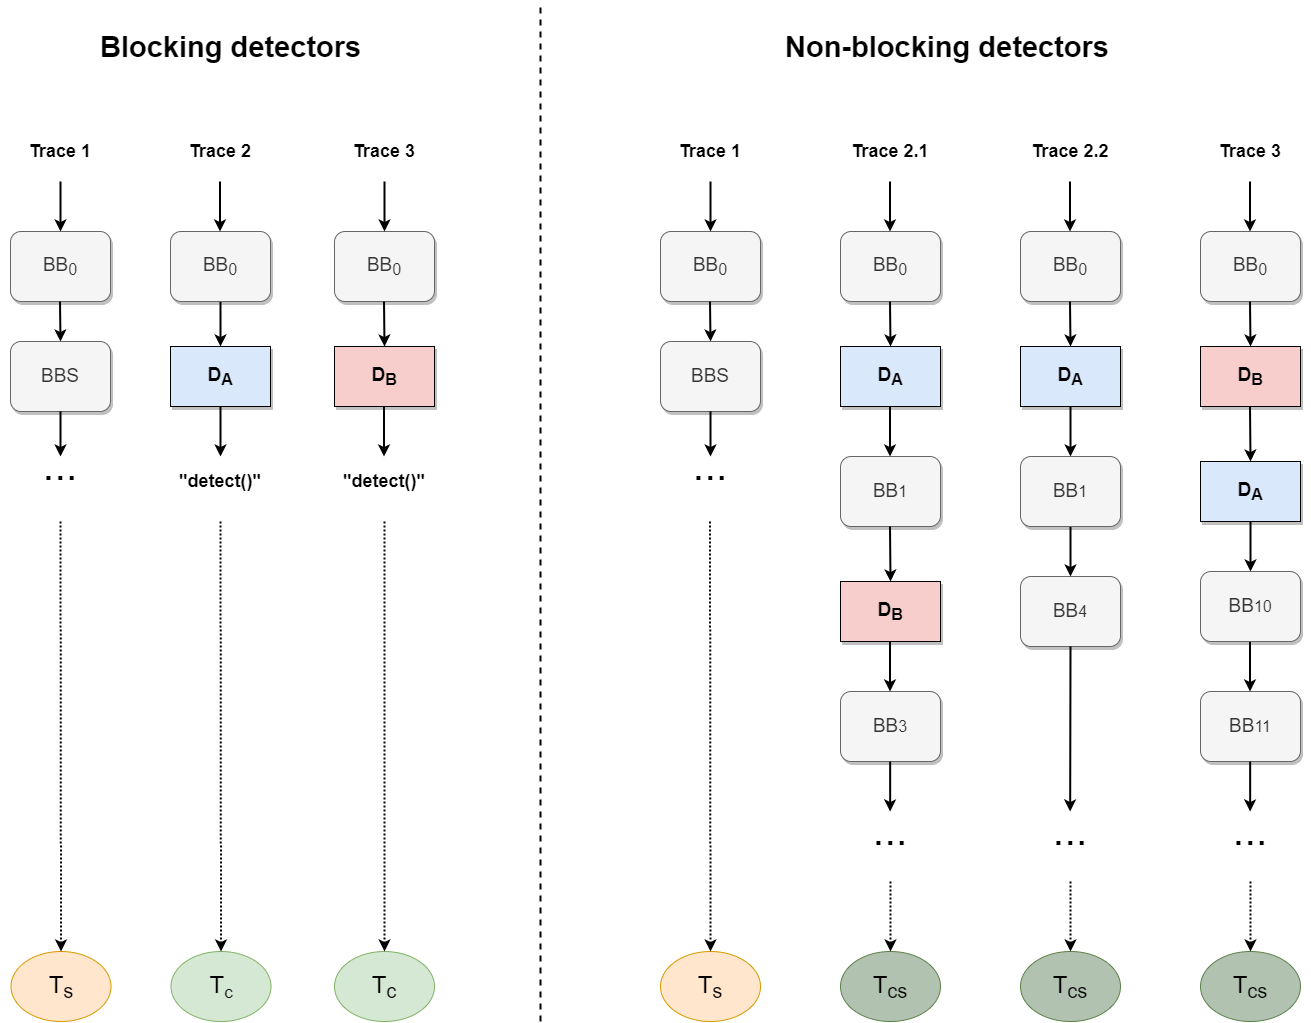
\includegraphics[scale=0.14]{img/CCP-prop-stopping2-en.drawio.png}
                \end{figure}
        }\only<3>{
                \begin{figure}
                    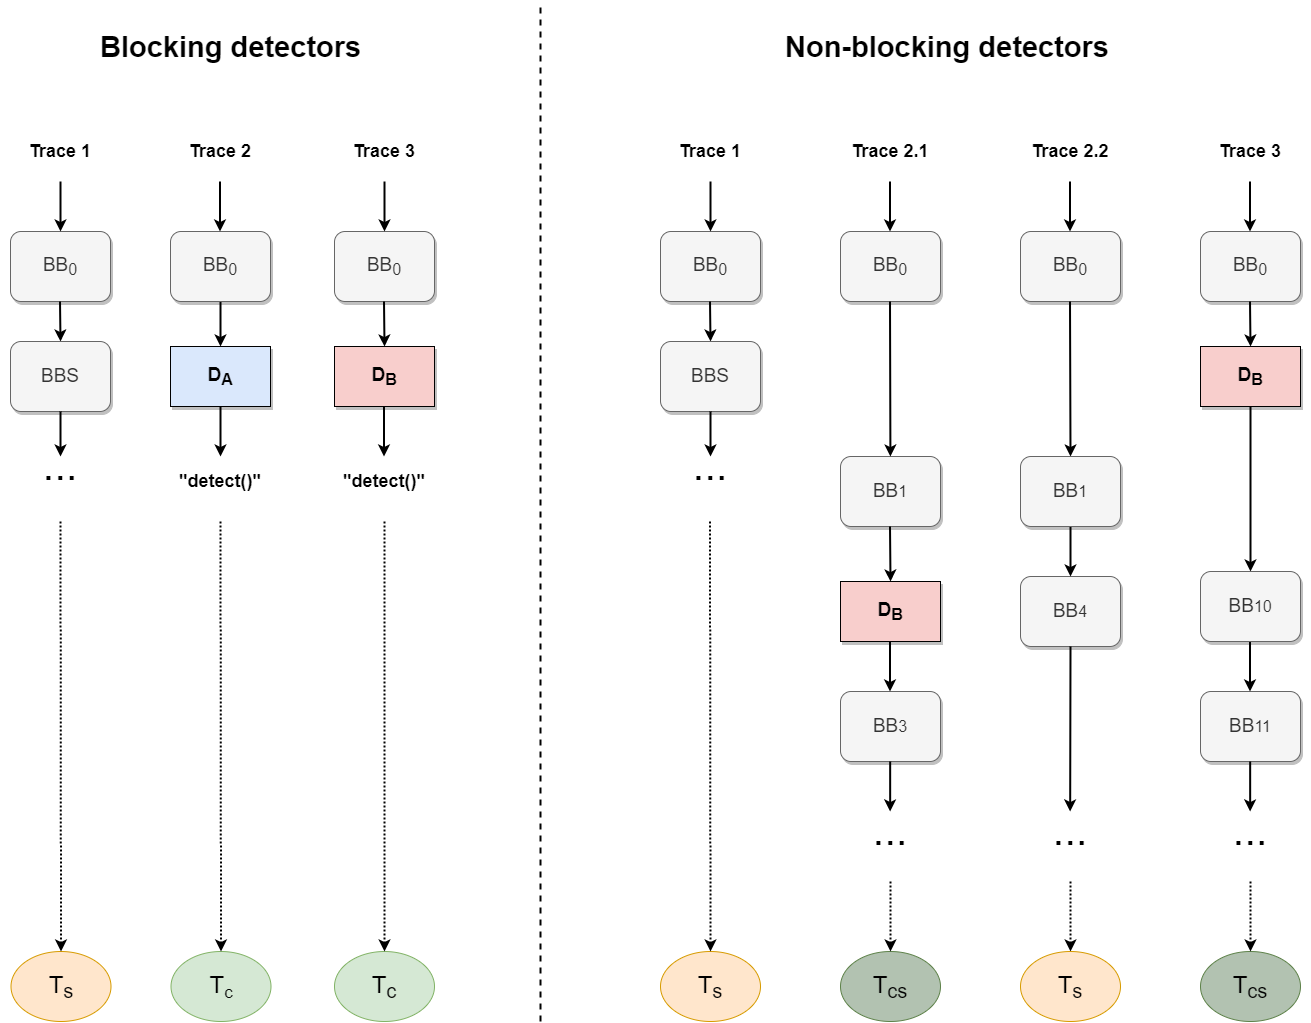
\includegraphics[scale=0.14]{img/CCP-prop-stopping2-en-DB.drawio.png}
                \end{figure}
        }\only<4>{
                \begin{figure}
                    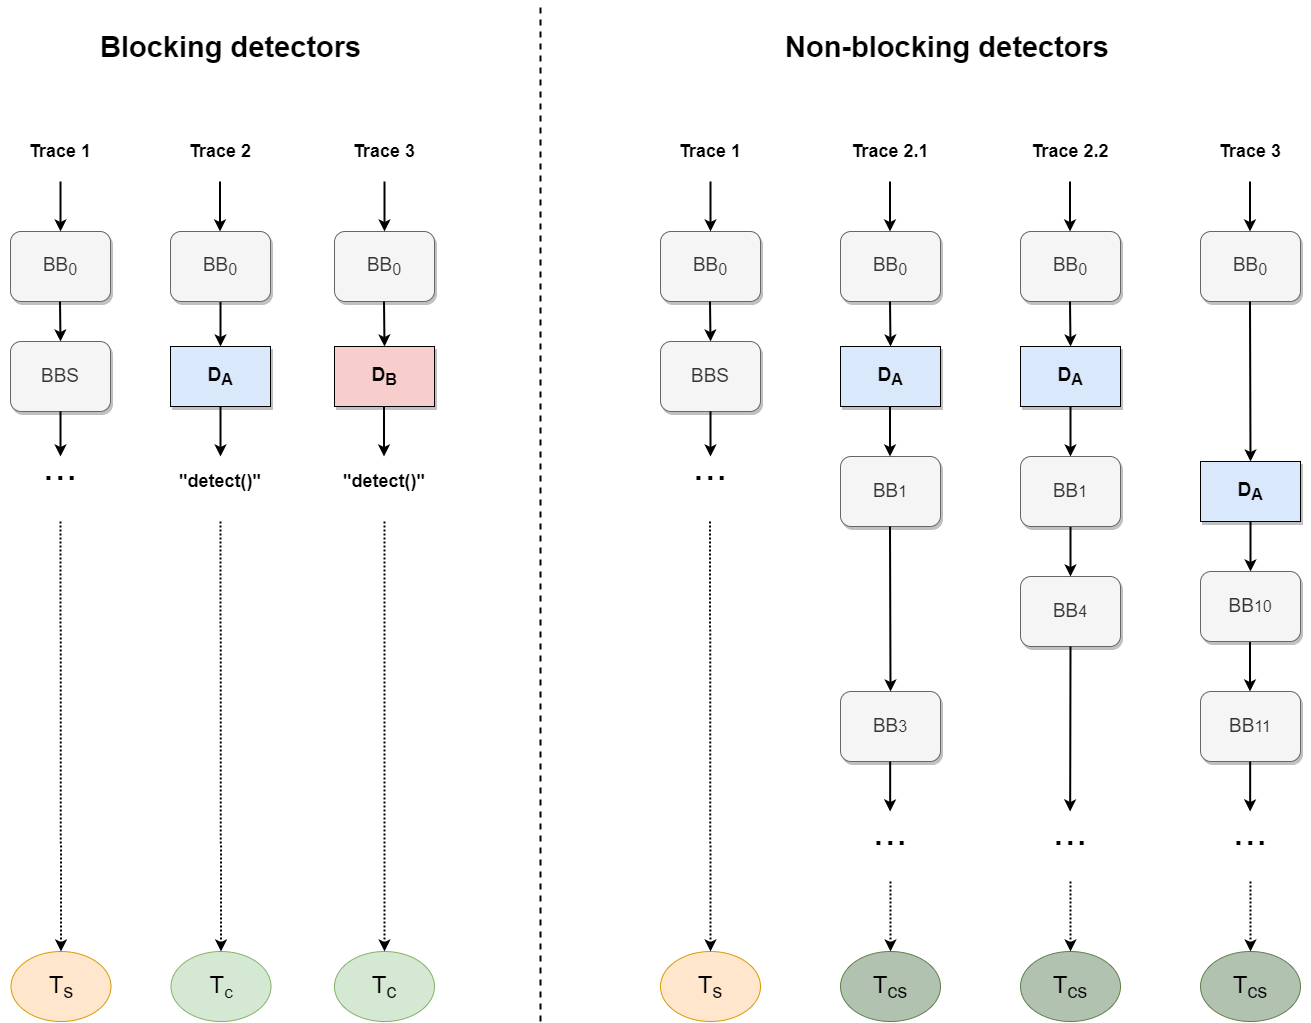
\includegraphics[scale=0.14]{img/CCP-prop-stopping2-en-DA.drawio.png}
                \end{figure}
        }
    \end{tiny}
\end{frame}

\begin{frame}[fragile]{Countermeasure optimization - Principle} 
    \begin{small}
        \begin{itemize}
            \item \textbf{An optimization problem:} Search the minimal set of detectors $\mathcal{D}$ such as at least one detector cover each trace of the set of detected attack traces
            \item[] $\Rightarrow$ using non-blocking detectors
            \item[] 
            \item[] 
            \item Exploration space can be reduced by \textit{classification} step:
            \begin{itemize}
                \item If $\forall t \in T', d_i \notin \{cm(t)\}$, $d_i$ is \textbf{inactive} (should be removed)
                \item If $\exists t \in T', cm(t) = \{d_i\}$, $d_i$ is \textbf{necessary} (should be kept)
                \item[] 
                \item Other detectors are \textbf{repetitive}
                \item[] $\Rightarrow$ focus on traces containing only \textbf{repetitive} detectors
            \end{itemize}
            \item[]            
        \end{itemize}
    \end{small}
\end{frame}

\begin{frame}[fragile]{Methodology - Step 1 - Test Duplication results in 2 faults}
    \textbf{VerifyPIN + Test Duplication:}
    \begin{itemize}
        \item[]
        \item 86 traces in 2 faults with \textbf{Lazart}
    \end{itemize}
    
    \begin{table}[]
        \caption{Detectors classification in 2 faults}
        \begin{tabular}{|l|l|l|l|l|l|l|l|l|l|l|l|}
            \hline
            \rowcolor[HTML]{C0C0C0} 
            Detector                           & 0 & 1                         & 2 & 3 & 4 & 5 & 6 & 7 & 8                         & 9                         & 100                       \\ \hline
            \rowcolor[HTML]{FFAC67} 
            \cellcolor[HTML]{C0C0C0}Class & R & \cellcolor[HTML]{FF8585}I & R & R & R & R & R & R & \cellcolor[HTML]{9AFF99}N & \cellcolor[HTML]{FF8585}I & \cellcolor[HTML]{9AFF99}N \\ \hline
        \end{tabular}
    \end{table}

    \begin{columns}
        \begin{column}{0.50\textwidth}
            \lstset{style=customc}
            \lstset{escapeinside={<@}{@>}}
            \begin{lstlisting}
bool verify_pin(uchar* user_pin) {
    if(try_counter > 0)      <@{\color{orange!80} \textbf{D0}}@> & <@{\color{red!80} \textbf{D1}}@>
        if(compare(user_pin, card_pin, PIN_SIZE)) {  <@{\color{OliveGreen} \textbf{D8}}@>
            try_counter = 3;
            return true;
        } else {  <@{\color{red!80} \textbf{D9}}@>
            try_counter--;
            return false;
        }
    return false;
}
            \end{lstlisting}
        \end{column}
        \begin{column}{0.5\textwidth}
            \lstset{style=customc}
            \lstset{escapeinside={<@}{@>}}
            \begin{lstlisting}  
bool compare(uchar* a1, uchar* a2, size_t size) {
    bool result = true;
    size_t i = 0;
    for(; i < size; i++) {  <@{\color{orange!80} \textbf{D2}}@> & <@{\color{orange!80} \textbf{D3}}@>
        if(a1[i] != a2[i]) {  <@{\color{orange!80} \textbf{D4}}@> & <@{\color{orange!80} \textbf{D5}}@>
            result = false; 
        }
    }

    if(i != size)  <@{\color{orange!80} \textbf{D6}}@> & <@{\color{orange!80} \textbf{D7}}@>
        countermeasure(100);  <@{\color{OliveGreen} \textbf{D100}}@>

    return result;
}
            \end{lstlisting}
    	\vfill
        \end{column}
    \end{columns}
\end{frame}

\begin{frame}[fragile]{Step 4 - Removed CCPs for verifyPIN (2 faults)}
	\vfill
    \begin{columns}
        \begin{column}{0.50\textwidth}
            \vspace{0.2cm}
            
            The {\color{Red}removed} and {\color{OliveGreen}kept} detectors and bodies for \textit{Test duplication} on \texttt{verify\_pin} with 2 faults
            \vspace{0.5cm}
    
            \lstset{style=customc}
            \lstset{escapeinside={<@}{@>}}
            \begin{lstlisting}
bool verify_pin(uchar* user_pin) {
    <@{\color{Red}bool c\_1;}@>
    <@{\color{OliveGreen}bool c\_2;}@>
    <@{\color{Blue}if}@>(<@{\color{Red}c\_1 = }@>try_counter > 0) {
        <@{\color{Red}if(!c\_1)}@>
            <@{\color{Red}killcard();}@>
            
        <@{\color{Blue}if}@>(<@{\color{OliveGreen}c\_2 = }@>compare(user_pin, card_pin, PIN_SIZE)) {
             <@{\color{OliveGreen}if(!c\_2)}@>
                <@{\color{OliveGreen}countermeasure();}@>
            try_counter = 3;
            <@{\color{Blue}return}@> true;
        } <@{\color{Blue}else}@> {
            <@{\color{Red}if(c\_2)}@>
                <@{\color{Red}countermeasure();}@>
            try_counter--;
            <@{\color{Blue}return}@> false;
        }
    } <@{\color{Red}else}@>
        <@{\color{Red}if(c\_1)}@>
            <@{\color{Red}countermeasure();}@>
    
    <@{\color{Blue}return}@> false;
}
            \end{lstlisting}
        \end{column}
        
        \begin{column}{0.5\textwidth}
            \lstset{style=customc}
            \lstset{escapeinside={<@}{@>}}
            \begin{lstlisting}
bool compare(uchar* a1, uchar* a2, size_t size) {
    bool result = true;
    <@{\color{Blue}size\_t}@> i = 0;
    <@{\color{OliveGreen}bool c\_1;}@>
    <@{\color{Red}bool c\_2;}@>
    <@{\color{Red}bool c\_3;}@>
    
    <@{\color{Blue}for}@>(; <@{\color{OliveGreen}c\_1 =}@> i < size; i++) { 
        <@{\color{Red}if(!c\_1)}@>
            <@{\color{Red}countermeasure();}@>
        <@{\color{Blue}if}@>(<@{\color{Red}c\_2 =}@> a1[i] != a2[i]) {
            <@{\color{Red}if(!c\_2)}@>
                <@{\color{Red}countermeasure();}@>
            result = false; 
        } <@{\color{Red}else}@>
            <@{\color{Red}if(c\_2)}@>
                <@{\color{Red}countermeasure();}@> 
    }
    <@{\color{OliveGreen}if(c\_1)}@>
        <@{\color{OliveGreen}countermeasure();}@>

    <@{\color{OliveGreen}if(}@><@{\color{Red}c\_3 = }@><@{\color{OliveGreen} i != size) \{}@>
        <@{\color{Red}if(!c\_3)}@>
            <@{\color{Red}countermeasure();}@>
        <@{\color{OliveGreen}countermeasure();}@>
    
    <@{\color{OliveGreen}\}}@> <@{\color{Red}else}@>
        <@{\color{Red}if(c\_3)}@>
           <@{\color{Red}countermeasure();}@>

    <@{\color{Blue}return}@> result;
}
            \end{lstlisting}
    	\vfill
        \end{column}
    \end{columns}
\end{frame}

\subsection{Experimentations}

\begin{frame}{Experimentations} 
    \begin{tiny}
        \begin{columns}
            \begin{column}{0.55\textwidth}
                \begin{table}[!t]
                    \centering
                    \label{tbl:ccpa-results}
                    \begin{tabular}{|l|c|c|c|c|}
                        \hline
                        Program       & \multicolumn{1}{l|}{Detectors} & \multicolumn{1}{l|}{1 attack} & \multicolumn{1}{l|}{2 attacks} & \multicolumn{1}{l|}{3 attacks} \\ \hline
                        VP + TD       & 11                       & 72\%                         & 63\%                          & 18\%                          \\ \hline
                        VP + SSCF     & 13                       & 92\%                         & 76\%                          & 23\%                          \\ \hline
                        VP + LBH       & 31                       & 93\%                         & 93\%                          & 32\%                          \\ \hline \hline
                        FU + TD       & 14                       & 0\%                          & 0\%                           & 0\%                           \\ \hline
                        FU + SSCF     & 24                       & 12\%                         & 12\%                          & 8\%                           \\ \hline \hline
                        GC1 + TD      & 39                       & 37\%                         & 34\%                          & 34\%                          \\ \hline
                        GC1 + SSCF    & 38                       & 57\%                         & 28\%                          & 28\%                          \\ \hline \hline
                        AES RK + TD   & 2                        & 50\%                        & 50\%                         & 0\%                         \\ \hline
                        AES RK + SSCF & 3                        & 66\%                        & 33\%                         & 0\%                         \\ \hline
                        AES C + TD    & 8                        & 50\%                         & 50\%                          & 0\%                           \\ \hline
                        AES C + SSCF  & 13                       & 76\%                         & 61\%                            & 38\%                             \\ \hline
                    \end{tabular}
                \end{table}
            \end{column}
        
            \begin{column}{0.5\textwidth}
                 Three countermeasures experimented:
                 \begin{itemize}
                     \item[]
                     \item \textit{Test duplication} (\textbf{TD}): presented previously
                     \item[]
                     \item \textit{SecSwift Control Flow} (\textbf{SSCF})\cite{Ferriere/LLVM19}: associates an unique identifier to each basic block and uses a xor-based mechanism to ensure that the correct branch has been taken
                     \item[]
                     \item \textbf{LBH} \cite{Lalande/ESORICS14}: introduce step counters to protect against C-level instruction skips. Each counter verification is a \texttt{detector}
                 \end{itemize}
            \end{column}
        \end{columns}
    \end{tiny}
\end{frame}

\section{Conclusion and future work}


%%%%%%%%%%%%%%%%%%%%%%%%%%%%%%%%%%%%%%%%%%%%%%%%%%%%%%%%%%%%%%%%%%%%%%%%
\begin{frame} \frametitle{Conclusion} 
{\small


    Robustness evaluation with Lazart
    \begin{itemize}
        \item filter of multi-fault attacks: equivalence and redundancy
        \item combination of fault models
        \item user accessibility, case studies
        \item[] 
    \end{itemize}

    Countermeasures evaluation
    \begin{itemize}
        \item isolation analysis
        \item placement algorithms
        \item[] $\rightarrow$ gives strong guarantees, even if the trace set is incomplete 
        \item[] $\rightarrow$ allows combination of fault model in multiple faults
        \item detector optimization algorithm
        \item[] $\rightarrow$ up to 80\% of \texttt{detectors} removed
        \item[]
    \end{itemize}

     
{\tiny
        \textbf{Publications:}
        \begin{itemize}
            \item \textit{Combining Static Analysis and Dynamic Symbolic Execution in a Toolchain to detect Fault Injection Vulnerabilities}
            \item[] Guilhem Lacombe, David Féliot, Etienne Boespflug and Marie-Laure Potet, \textit{Journal of Cryptography Engineering 2023}
            \item[]
            \item \textit{Combining Static Analysis and Dynamic Symbolic Execution in a Toolchain to detect Fault Injection Vulnerabilities}
            \item[] Guilhem Lacombe, David Féliot, Etienne Boespflug and Marie-Laure Potet, \textit{PROOFS Workshop 2021}
            \item[]
            \item \textit{Countermeasures Optimization in Multiple Fault-Injection Context}
            \item[] Etienne Boespflug, Cristian Ene, Marie-Laure Potet and Laurent Mouniter, \textit{FDTC 2020}
        \end{itemize}
}
\vfill
}
\end{frame}

%%%%%%%%%%%%%%%%%%%%%%%%%%%%%%%%%%%%%%%%%%%%%%%%%%%%%%%%%%%%%%%%%%%%%%%%
\begin{frame} \frametitle{Future Works} 
{\tiny


    Tools:
    \begin{itemize}
        \item Extension of fault models in Lazart
        \item Extension of automated countermeasures in Lazart
        \item Validate contribution on more example programs
        \item Combination with static analysis
        \item "fault-aware" dynamic-symbolic execution engine
        \item [] 
    \end{itemize}
    
    \onslide<2->{
    Countermeasure placement:
    \begin{itemize}
        \item Study of countermeasures without IP granularity
        \item Study of countermeasures propagating states (SSCF, Swift...)
        \item[] $\rightarrow$ may require to consider two isolation analysis cases: sane CM's inputs and corrupted CM's inputs
        \item Study of more complex CFG fault models
        \item [] $\rightarrow$ requires to take into account the several entry and output points of the protection scheme
        \item Extension of notion of \textit{adequation}, \textit{perfection} of CMs and \textit{protectability} of fault models
        \item[] 
    \end{itemize}
    }
    
    \onslide<3->{
    Countermeasure optimization:
    \begin{itemize}
        \item Switch to Lazart 4
        \item Fully symbolic version (relax constraints on detectors)
        \item[] $\rightarrow$ internal states may be difficult to consider
        \item Study of other countermeasures
        \item[] 
    \end{itemize}
    }

\vfill
}
\end{frame}

\begin{comment}
%%%%%%%%%%%%%%%%%%%%%%%%%%%%%%%%%%%%%%%%%%%%%%%%%%%%%%%%%%%%%%%%%%%%%%%%
\begin{frame} \frametitle{Future Works} 
{\tiny


\begin{columns}
        
    \begin{column}{0.3\textwidth}
    Implementation:
    \begin{itemize}
        \item Extension of fault model in Lazart
        \item Extension of automated countermeasures in Lazart
        \item Validate contribution on more example program
        \item Binary level implementation
        \item [] 
        \item[] 
        \item[] 
        \item[] 
    \end{itemize}
    \end{column}
    
    \begin{column}{0.4\textwidth}
    \onslide<2->{
    Countermeasure placement
    \begin{itemize}
        \item Study of countermeasures without IP granularity
        \item Study of countermeasures propagating states 
        \item[] $\rightarrow$ may require to consider two isolation analysis cases: sane CM's inputs and corrupted CM's inputs
        \item Study of more complex fault models
        \item [] $\rightarrow$ requires to take into account the several entry and output points of the protection scheme
        \item Study of incomplete catalogs
        \item[] 
    \end{itemize}
    }
    \end{column}
    
    \begin{column}{0.4\textwidth}
    \onslide<3->{
    Countermeasure optimization
    \begin{itemize}
        \item Fully symbolic version (relax constraints on detectors)
        \item How to protect detectors with other fault models ?
        \item Over-approximation approaches 
        \item[] 
        \item[] 
        \item[] 
        \item[] 
        \item[] 
    \end{itemize}
    }
    \end{column}
    
        
\end{columns}
\vspace{0.2cm}

\vfill
}
\end{frame}
    
\end{comment}


%%%%%%%%%%%%%%%%%%%%%%%%%%%%%%%%%%%%%%%%%%%%%%%%%%%%%%%%%%%%%%%%%%%%%%%%
\begin{frame}[fragile, noframenumbering] \frametitle{The End} 
\vspace{1cm}
\begin{center}
    {\large Thanks for watching}
\end{center}
\vfill
\end{frame}

\begin{comment}

\subsection{Conclusion}

%%%%%%%%%%%%%%%%%%%%%%%%%%%%%%%%%%%%%%%%%%%%%%%%%%%%%%%%%%%%%%%%%%%%%%%%
\begin{frame}[fragile] \frametitle{Conclusion} 
\begin{itemize}
    \item A methodology to \textit{optimize} program protected by \textit{side-effect free} detectors (up to 80\% of \texttt{detectors} removed)
    \item[]
    \item Only one program exploration $\rightarrow$ realistic analysis time for real world programs
    \item[]
    \item The methodology is generic regarding to the analysis level and trace generation method
    
\end{itemize}
\vfill
\end{frame}



\subsection{Conclusion}
%%%%%%%%%%%%%%%%%%%%%%%%%%%%%%%%%%%%%%%%%%%%%%%%%%%%%%%%%%%%%%%%%%%%%%%%
\begin{frame} \frametitle{Conclusion} 
{\small

\begin{itemize}
    \item Robustness of placement depend on the property of the catalog
    \item[]
    \item P' is guaranteed as robust if the required protection coefficients (K) are available
    \item[] $\rightarrow$ if not, attack traces on P' are known
    \item []$\rightarrow$ more robust than P even if trace set is incomplete
    \item[]
    \item Optimal placement is guaranteed with ILP
    \item[]
    \item Protection weight: $rep < bloc < min < atk < naive$ 
    \item[]
\end{itemize}

            \begin{table}[h]
                {\tiny
                \begin{center}%\setlength\tabcolsep{1.5pt}
\begin{tabular}{l|l|ll|l|lll}
Algorithme & Type & \multicolumn{2}{l|}{Guarantees $P'$} & Complexity & \multicolumn{3}{l}{Required analysis} \\
 &  & Robust & Optimal &  & AA & Red & HS \\
 \hline
naive & syst. & \checkmark & - & $O(t)$ & \checkmark & - & - \\
atk & syst. & \checkmark & - & $O(t)$ & \checkmark & - & - \\
min & syst. & \checkmark & - & $O(t)$ & \checkmark & \checkmark & - \\
bloc-h & bloc & \checkmark & - & $O(t)$ & \checkmark & \checkmark & \checkmark \\
rep-opt & distributed & \checkmark & \checkmark & NP-Complete & \checkmark & \checkmark & - \\
\end{tabular}
                \end{center} 
                }
                \end{table}
    

\begin{itemize}
    \item Placement algorithm is slow compared to DSE and redundancy analysis
    \item[] $\rightarrow$ event with optimal algorithm and ILP (1-fault attacks)
\end{itemize}
}
\vfill
\end{frame}


%%%%%%%%%%%%%%%%%%%%%%%%%%%%%%%%%%%%%%%%%%%%%%%%%%%%%%%%%%%%%%%%%%%%%%%%
\begin{frame} \frametitle{Future Works} 
{\small



\begin{itemize}
    \item Study of countermeasures without IP granularity
    \item[]
    \item Study of countermeasures propagating states 
    \item[] $\rightarrow$ may require to consider two isolation analysis cases: sane CM's inputs and corrupted CM's inputs
    \item[]
    \item Study of more complex fault models
    \item [] $\rightarrow$ requires to take into account the several entry and output points of the protection scheme
    \item[]
    \item Study of incomplete catalogs
\end{itemize}

\vfill
}
\end{frame}
\end{comment}


\section*{}

\miniframesoff

\begin{frame}[fragile, noframenumbering]{Lazart architecture} 
    \begin{figure}
        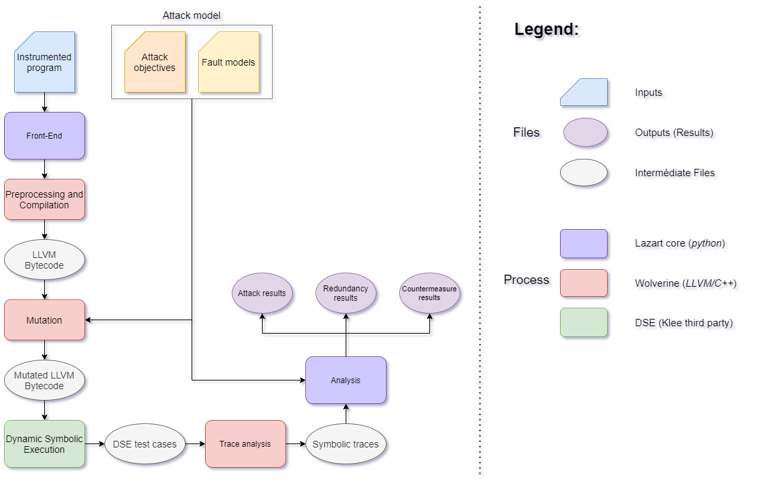
\includegraphics[width=\textwidth]{img/lazart-arch.png}
    \end{figure}
\end{frame}
    
\begin{frame}[fragile, noframenumbering]{Model protectability} 
    \begin{tiny}
        \begin{figure}
            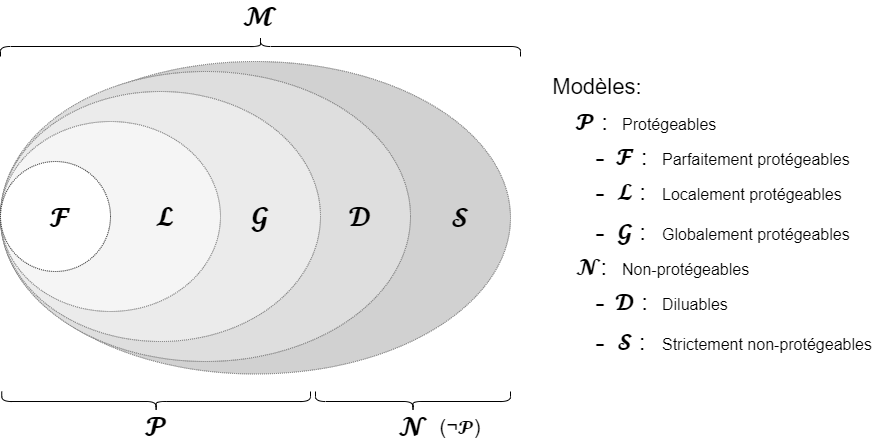
\includegraphics[scale=0.32]{img/protectable-models-set-extended.drawio.png}
        \end{figure}

        \begin{itemize}
            \item notion of \textit{adequation} of CMs
            \item notion of \textit{perfection} of CMs
            \item notion of protectability of models
        \end{itemize}
        \vfill
    \end{tiny}
\end{frame}

\begin{frame}[fragile, noframenumbering] \frametitle{Future work - Fully symbolic CCPO} 
    \begin{itemize}
        \item The methodology requires properties for detectors $\rightarrow$ a full symbolic version can be used
        \item[]
        \item Each detectors forks the execution:
        \lstset{style=customc}
        \begin{lstlisting}
if(sym_bool()) // Is the detector active ?
{
    // Local code with detector
}
else
{
    // Local unprotected code.
}
        \end{lstlisting}
        \item[]
        \item Issues:
        \begin{itemize}
            \item Paths explosion
            \item Some countermeasure structures depend on the presence of detectors (can require specific instrumentation for CMs)
        \end{itemize}
        \item[]
    \end{itemize}
\vfill
\end{frame}

\begin{frame}[fragile, noframenumbering]{Detector requirements} 
    \begin{itemize}
       \item[] Let $V_P$ be the state of the non-protected program and $V_C$ the state of the countermeasures.
       \item[] The detector has limitation for the read and write operation on the states $V_P$ et $V_C$.
    \end{itemize}
    
    \lstset{style=customc}
    \lstset{escapeinside={<@}{@>}, caption=Generic detector example}
    \begin{lstlisting}
...
stm1; // can: read(VP, VC) & write(VP, VC)

// Detector:
if(cond) { // read(VP, VC)
    stm2; // read(VP, VC) & write(VP, VC)
    killcard(); 
} 

stm3; // read(VP, VC) & write(VP, VC)
...
    \end{lstlisting}
\end{frame}

\begin{frame}[fragile, noframenumbering]{\texttt{memcmps3} program} 
    \begin{columns}
        \begin{column}{0.5\textwidth}
            \lstset{style=customc}
            \lstset{escapeinside={<@}{@>}, caption=Analysis's \texttt{main}}
            \begin{lstlisting}
// main.c
#include "lazart.h"
#include "memcmps.h"

#define SIZE 4

int main()
{  
    // Inputs
    uint8_t a1[SIZE];
    _LZ__SYM(a1, SIZE); // Symbolic array
    uint8_t a2[SIZE];
    _LZ__SYM(a2, SIZE); // Symbolic array
    
    bool equals = true;
    for(size_t i = 0; i < SIZE; ++i)
        if(a1[i] != a2[i])
            equals = false;
    _LZ__ORACLE(!equal); // Consider only different inputs
    
    BOOL res = memcmps(a1, a2, SIZE); // Call studied function

    _LZ__ORACLE(res == TRUE); // Attack objective
}
            \end{lstlisting}
        \end{column}
        \begin{column}{0.5\textwidth}
            \lstset{style=customc}
            \lstset{escapeinside={<@}{@>}, caption=\texttt{memcmps3} program}
            \begin{lstlisting}
// memcmps.h
typedef BOOL uint16_t;
#define TRUE    0x1234u
#define FALSE   0x5678u
#define MASK    0xABCDu

// memcmps.c
#include "memcmps.h"

BOOL memcmps(uint8_t* a, uint8_t* b, size_t len)
{
  BOOL result = FALSE;
  
  if (!memcmp(a, b, len)) {
    result ^= MASK;           // result = FALSE ^ MASK
    if (!memcmp(a, b, len)) {
      result ^= FALSE ^ TRUE; // result = MASK ^ TRUE
      if (!memcmp(a, b, len)) {
        result ^= MASK;       // result = TRUE
      }
    }
  }

  return result;
}
            \end{lstlisting}
        \end{column}
    \end{columns}
\end{frame}

\begin{frame}[fragile, noframenumbering]{\texttt{memcmps3} analysis file} 
    \lstset{style=custompython}
    \lstset{escapeinside={<@}{@>}, caption=\texttt{memcmps3} program}
    \begin{lstlisting}
#!/usr/bin/python3
from lazart.lazart import *

attack_model = functions_list(["memcmps"], [ti_model(), data_model({ "vars": { "result": "__sym__", "len":  "__sym__" } })])

a = Analysis(["memcmps.c", "main.c"], # Input files 
    attack_model, # Attack model
    flags=AnalysisFlag.AttacksAnalysis, # Analysis type
    compiler_args="-Wall",
    max_order=4,
    path="my_analysis")

execute(a)
    \end{lstlisting}
\end{frame}

\begin{frame}[fragile, noframenumbering]{Countermeasure optimization} 
    \begin{small}
        \begin{itemize}
            \item The program $P$ contains a set of \textit{detector} $\mathcal{D}$. 
            \item[]
            \item[] Stopping traces: $s_0 ... s_n d_i$, where $s_i$ are nominal or faulty transitions, and $d_i$ the triggered detector
            \item[] Non-stopping traces: $s_0 ... s_n d_i s^2_0 ... s^2_n d_j ...$ with $d_i$ detectors triggering
            \item[] $\rightarrow$ Stopping traces are prefix of non-stopping ones. One stopping trace can lead to several non-stopping traces
            \item [] 
            \item \textbf{Goal} $\Rightarrow$ find the minimal set of detectors in which at least one detector is kept for each trace
            \item [] 
            \item Only traces which validate the attack objective $\phi$ and in which at least one detector is triggered are considered. This trace set is denoted $\mathcal{T}_P$.
            \item[] The detector \textit{selection} is an optimization problem, searching a minimal set of detectors covering each traces of $\mathcal{T}_P$ with at least one trigger.
            \item[] Exploration space can be reduced:
            \begin{itemize}
                \item If $\forall t \in T', d_i \not\in  \{triggered(t)\}$, $d_i$ is inactive (should be removed)
            \item If $\exists t \in T', triggered(t) = \{d_i\}$, $d_i$ is necessary (should be kept)
            \end{itemize}
        \end{itemize}
    \end{small}
\end{frame}

\begin{frame}[noframenumbering]{Experimentation results - Playing with the attack objectives} 
    \only<1>{
        \vspace{0.6cm}
        The \textbf{attack objective} strongly impacts the removed \textbf{detectors}.
        
        \begin{itemize}
            \item []
            \item $\phi_{auth}$: being authenticated with a false PIN.
            \item $\phi_{ptc}$: do not decrement the try counter with a false PIN.
        \end{itemize}
        
        \begin{center}    
            \begin{table}[!t]
                \caption{Removed detectors depending on attack objective (VP + TD)}
                \centering
                \label{tbl:oracles}
                \begin{tabular}{|l|c|c|c|}
                    \hline
                    Property     & \multicolumn{1}{l|}{1 fault} & \multicolumn{1}{l|}{2 faults} & \multicolumn{1}{l|}{3 faults} \\ \hline
                    $\phi_{auth}$         & 83\%                         & 72\%                          & 18\%                          \\ \hline
                    $\phi_{ptc}$          & 72\%                         & 63\%                          & 9\%                           \\ \hline
                    $\phi_{auth\; \wedge \;ptc}$ & 83\%                         & 72\%                          & 18\%                          \\ \hline
                    $\phi_{auth\; \vee \;ptc}$  & 72\%                         & 63\%                          & 9\%                           \\ \hline
                    $\phi_{true}$         & 18\%                         & 9\%                           & 9\%                           \\ \hline
                \end{tabular}
            \end{table}
        \end{center}
        \vfill
    }
\end{frame}

\begin{frame}[fragile, noframenumbering]{Test Duplication} 
    The \textit{Test Duplication} generate two detectors for each conditional branch.

    \vspace{0.5cm}

    \begin{figure}
        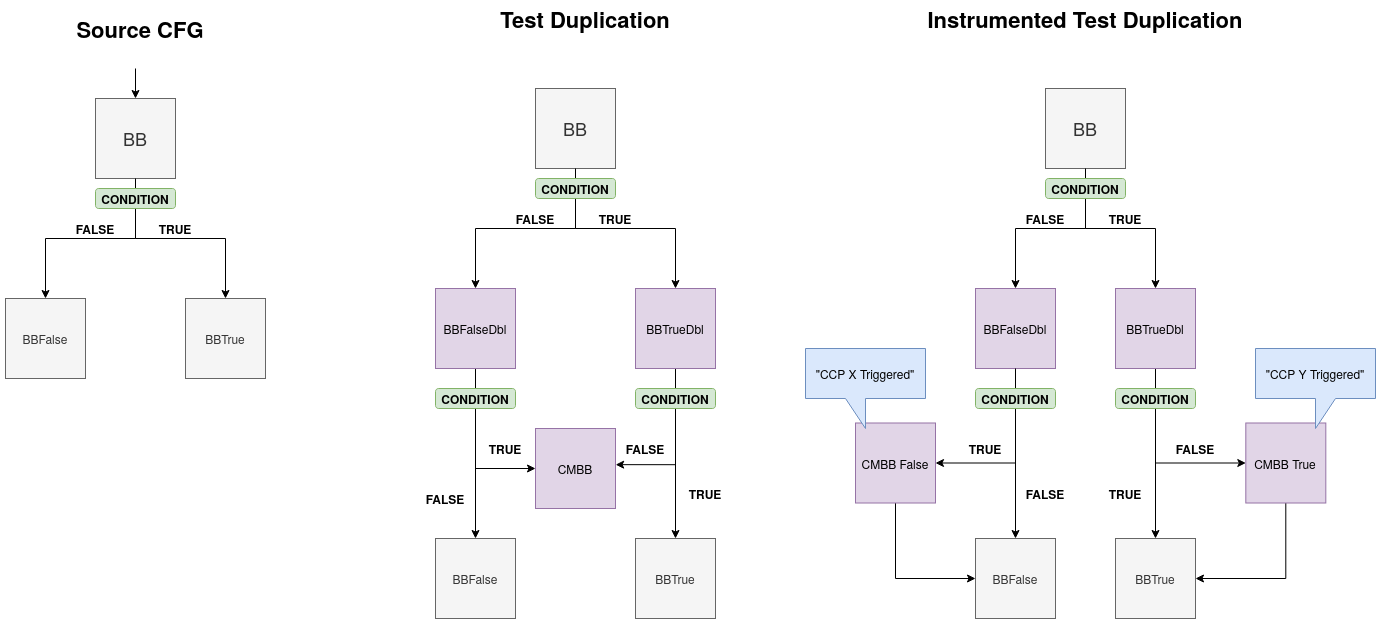
\includegraphics[scale=0.2]{img/test-duplication-scheme-complete-old.png}
    \end{figure}
\end{frame}

\begin{frame}[fragile, noframenumbering]{SecSwift Control-Flow} 
    \begin{figure}
        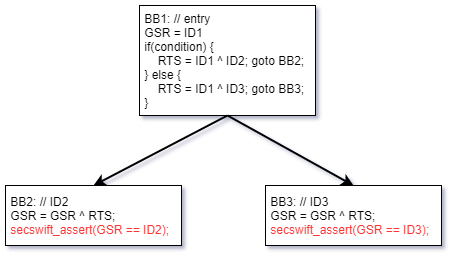
\includegraphics[scale=0.3]{img/secswift-CF.png}
    \end{figure}
    
    \begin{itemize}
        \item []
        \item[] SecSwift ControlFlow is one of the 3 parts of SecSwift\cite{Ferriere/LLVM19}
        \item []
        \item Designed for Control-Flow Integrity (CFI)
        \item[]
        \item Uses static signature for each basic block and propagate errors
        \item[]
        \item Each \lstinline{secswift_assert} is a \emph{detector}
    \end{itemize}
    \vfill
\end{frame}

\begin{frame}[fragile, noframenumbering]{LBH's countermeasure \cite{Lalande/ESORICS14}} 
    \vspace{0.3cm}
    
    \lstset{style=customc}
    \lstset{escapeinside={<@}{@>}}
    \begin{lstlisting}
#define <@{\color{red!95} INCR}@>(cnt,val)  cnt = cnt + 1;
#define <@{\color{red!95} CHECK\_INCR}@>(cnt,val, cm_id) if(cnt != val) countermeasure(cm_id); \
    cnt = cnt + 1;
[...]
        
        
BOOL verifyPIN(<@{\color{red!95}unsigned short* CNT\_0\_VP\_1}@>) 
{
    <@{\color{red!95} CHECK\_INCR(*CNT\_0\_VP\_1, CNT\_INIT\_VP + 0, 0LL)}@>
    g_authenticated = 0;
    <@{\color{red!95} CHECK\_INCR(*CNT\_0\_VP\_1, CNT\_INIT\_VP + 1, 1LL)}@>
    <@{\color{red!95} DECL\_INIT(CNT\_0\_byteArrayCompare\_CALLNB\_1, CNT\_INIT\_BAC)}@>
    <@{\color{red!95} CHECK\_INCR(*CNT\_0\_VP\_1, CNT\_INIT\_VP + 2, 2LL)}@>
    BOOL res = byteArrayCompare(g_userPin, g_cardPin, PIN_SIZE<@{\color{red!95}, \&CNT\_0\_byteArrayCompare\_CALLNB\_1}@>);
[...]
    \end{lstlisting}

    \begin{itemize}
        \item Insert \textit{step-counters} for each C construct
        \item[]
        \item \textit{Checking macros} (such as \lstinline{CHECK_INCR}) are \emph{detectors}
        \item[]
        \item Analysis allows to know where the counter verification can be removed
    \end{itemize}
    \vfill
\end{frame}

\miniframesoff
\begin{frame}[allowframebreaks, noframenumbering]{References}
   \nocite{*}   
 
    {\footnotesize 
        \bibliography{lib/biblio}{} 
        \bibliographystyle{unsrt}
    }
    \vfill
\end{frame}

\end{document}

